\documentclass[article,type=msc,colorback,accentcolor=tud2a]{tudthesis}
%\documentclass[article,type=msc,colorback,accentcolor=tud2a]{tudreport}

%%%%%%%%%%%%%%%%%%%%%%%%%%%%%%%%%%%%%%%%%%%%%%%%%%%%%%%%%%%%%%%%%%%%%%%
%\usepackage{ngerman}

%%%%%%%%%%%%%%%%%%%%%%%%%%%%%%%%%%%%%%%%%%%%%%%%%%%%%%%%%%%%%%%%%%%%%%%

\newcommand{\getmydate}{%
  \ifcase\month%
    \or Januar\or Februar\or M\"arz%
    \or April\or Mai\or Juni\or Juli%
    \or August\or September\or Oktober%
    \or November\or Dezember%
  \fi\ \number\year%
}

\usepackage{masterthesis}

%selective compilation of files
\includeonly{./tex/masterthesis.fundamentals,./tex/masterthesis.seg,./tex/masterthesis.cpld}

\begin{document}
\thesistitle{Implementation and Performance Analyses of a Highly Efficient Algorithm for Pressure-Velocity Coupling}{Implementierung und Untersuchung einer hoch effizienten Methode zur Druck-Geschwindigkeits-Kopplung}
%\title{Implementation and Performance Analyses of a Highly Efficient Algorithm for Pressure-Velocity Coupling}{Implementierung und Untersuchung einer hoch effizienten Methode zur Druck-Geschwindigkeits-Kopplung}
  \author{Fabian Gabel}
  \referee{Prof. Dr. rer. nat. Michael Schäfer}{Dipl.-Ing Ulrich Falk}
  \department{Studienbereich CE}
  \group{FNB}
% \tuprints{12345}{1234}
  \makethesistitle
% \maketitle
  \selectlanguage{ngerman} \affidavit{Fabian Gabel} \selectlanguage{english}
  \tableofcontents
  \listoffigures
  \listoftables
  \listofalgorithms

    \nomenclature{$x_i, i \in \{1,2,3\}$}{Cartesian coordinates}
    \nomenclature{$t$}{Time}
    \nomenclature{$V$}{Volume}
    \nomenclature{$S$}{Surface}
    \nomenclature{$\rho$}{Density}
    \nomenclature{$u_i, i \in \{1,2,3\} $}{Cartesian velocity components}
    \printnomenclature



  \section*{TODO LIST}

  \begin{itemize}
    \item change the matrix coefficient indexing to \(a_P^{u_i,p}\) like in \cite{darwish09}.
    \item extend nomenclature
    \item align equations using the \textbf{alignat} environment
    \item check pressure correction equation on iteration indices (gradients)
    \item check simple chapter, since the right hand side lacks of deferred corrector and under-relaxed velocities
    \item mention the boundary conditions for the pressure correction
    \item extend algorithms to handle passive scalars
    \item check all headings for correct spelling
    \item mention that for an unknown velocity field the partial differential equation for the temperature is non-linear as well
    \item consistent use of either temperature or energy equation
    \item check the signs in the Boussinesq approximation
    \item pressure weighted interpolation method for large body forces?
    \item not only speed but also improvement of robustness
    \item instationary flows?
    \item align exponents in the equation for the Newton-Raphson linearization
    \item use temperature-TO-velocity coupling
  \end{itemize}

  \section{Introduction}

The growing involvement of numerical methods in sciences and industrial practice due to the advances in computer architecture and algorithms has had a great impact on academic research and industrial development processes in the past decades. Numerical methods nowadays form an integral part in forming a better understanding of physical phenomena and modelling the behaviour of technical systems besides purely theoretical or experimental approaches. Especially numerical methods for the simulation of fluid flow, also known as \emph{CFD} (\emph{Computational Fluid Dynamics}), have continuously been creating new challenges for the ongoing process of hardware and software improvements. Not only more complexity has to be reflected in computational methods to solve fluid flow problems but also less time to generate results is preferable to accelerate development processes. Parallel computing on high performance computer clusters represents an additional field of study since many numerical methods rely on hardware requirements that cannot be met by office workstations. As are the fields of study, the possibilities to further increase performance of scientific applications are manifold. Advancements in numerical methods and mathematical models, programming paradigms and tailored libraries for new computer architectures that use the hardware to full capacity and the new hardware itself contribute to the continuous expansion of the boundaries of what is \emph{computable}.

The incompressible Navier-Stokes equations represent the commonly used mathematical model for incompressible flows. Among other properties this model incorporates a coupling between the involved variables velocity and pressure. Algorithms that tend to solve for incompressible flow fields thus have to address the so called pressure-velocity coupling. A common approach is to resolve this coupling through segregated solution methods. With this methods the algebraic equations for each of the dependent variables are solved sequentially using approximate values for the other involved variables. Achieving inter variable coupling is part of an iterative solution process such that in the end the solution field will fulfill all involved equations. One common representative of this type of algorithms is the SIMPLE algorithm that has been widely used in scientific codes or industrial solvers due to its small memory requirements. Reference \cite{acharya07} reviews the evolution of this type of algorithms.

The use of segregated solution algorithms comes with significant drawbacks. To stabilize the iteration for the coupling process, the obtained solutions have to be under relaxed, where the amount of under relaxation is furthermore dependent on the problem to be solved. Not only does this degrade the solver performance, but also there don't exist exist strict rules for the optimal choosing of the under relaxation. The resolution of the pressure-velocity coupling forms an essential part for the performance of a flow solver and hence creates the need for new coupling algorithms that are more robust or even independent of parameters and at the same time resource efficient in their application. An analysis of the pressure-velocity coupling can be found in \cite{peric90}.

One alternative approach to pressure-velocity coupling is by the simultaneous solution of the momentum and mass balance equations on co-located grids has been used in \cite{chen10,darwish09,falk13,galpin86,klaij13,mangani14,vakilipour12}. It was shown that the principal advantages of coupled solution approaches complement the drawbacks of segregated solution algorithms. Not only the computational time was reduced, also the robustness of the solution algorithm was increased. According to \cite{darwish09} no under relaxation was necessary to obtain a robust implementation. 

So far only \cite{galpin86,vakilipour12} additionally coupled a temperature equation to the two-dimensional Navier-Stokes equations and investigated the impact of different methods to achieve implicit temperature-to-velocity/pressure coupling on the solver performance. The objectives of the present thesis are to implement a fully coupled solution algorithm for the three-dimensional Navier-Stokes equations and the temperature equation and analyse their single and multi-processor performance.

The thesis begins by introducing the mathematical and physical fundamentals of flow problems. In this first chapter the main frame of partial differential equations to be solved numerically is introduced. Each subsection presents a brief derivation from the continuum mechanical point of view and presents common or necessary simplifications. This embraces not only a presentation of the Navier-Stokes equations for incompressible fluids but also the Boussinesq approximation that is widely used for incompressible flows that experience buoyant forces.

The third section outlines the fundamentals of finite-volume methods in general. At first the necessary terminology for numerical grids is established. Then the main approximation principles for the discretization of integral or differential operators are introduced. Since in the present thesis no further requirements are demanded other than grid structure one subsection gives an overview over common methods to handle non-orthogonal grids. The chapter concludes with presenting the main method of linearization for the Navier-Stokes equations used throughout the work.

The fourth section focusses on segregated solution methods as many ideas of the commonly used SIMPLE algorithm are relevant for the implementation of coupled solution methods. The section starts by discretizing the mass balance coming directly from the continuum mechanical introduction of the first section outlining its drawbacks on their applicability on co-located variable arrangements. The following sections then first introduce a remedy to the checker-boarding effect that would surge from an unmodified discretization of the mass balance by introducing a modification of the commonly used Rhie-Chow \cite{rhie82} momentum interpolation scheme. This modification is proven to yield results that do not depend on under-relaxation which is important for later comparison studies with the coupled solution algorithm. Then the popular SIMPLE algorithm is derived using the previously demonstrated interpolation scheme as basis for the construction of a pressure correction equation. In the following subsections the pressure equation and the two remaining sets of equations, the three momentum balances and the temperature equation, are discretized. Each section concludes with a complete list of the resulting discretized equations and calculations of the coefficients as they are implemented in the developed solver framework. The next subsections are dedicated to the implementation of boundary conditions. For each boundary condition, including the treatment of block boundaries the necessary modifications to the discretized equations are presented. Since in most of the cases the boundary conditions lead to a singular system for the pressure correction special the following chapter describes methods to constrain the pressure in incompressible flows. The section concludes by presenting the non-zero structure of the resulting assembled linear system, taking into account the special treatment of block boundaries with hanging nodes.

The structure of the fifth section, which describes the implemented coupled solution algorithm, is similar to the third section, since both solution approaches share a great part of their components. This is why special emphasize lays on pointing out the differences between both algorithms. The first subsection of this section therefore is a revision of the pressure velocity coupling that accounts for the implicit consideration of the pressure in the momentum balances. A major difference to segregated solution methods is then presented in the subsequent section and subsections: the coupling to the temperature equation. Here, different methods, varying in there relation of implicit and explicit coupling of velocities, pressure and temperature are derived. Then the necessary modifications for boundary conditions are presented. The final subsection presents the final form of the discretized equations and the resulting structure of the assembled linear systems with special emphasize on the effects of the different methods to achieve coupling of the velocities to the temperature equation and vice versa.

In section six the during this thesis developed \emph{CAFFA} (\emph{Computer Aided Fluid Flow Analysis}) framework is introduced for which the preceding chapters present the theoretical basis. The framework is linked to the PETSc library, a sophisticated framework for the parallelisation of solver applications as they surge in scientific computing and a set of efficient preconditioners and Krylov subspace solvers for the solution of linear systems. The following sections then introduce the building blocks of the framework, beginning with a grid generator for arbitrarily refined block structured grids and a preprocessor program ending with implementation details of the CAFFA solver. These details embrace the used message passing model, the control of convergence and the domain composition in the context of parallel computations.

After the implementation has been described, section seven presents the conducted study to assure the verification of the CAFFA framework. After brief introduction in the theory behind the verification of scientific codes via manufactured solutions is given, an own manufactured solution for the Navier-Stokes equations using the Boussinesq approximation is proposed followed by the results of an grid convergence study to prove the order of accuracy of the developed solvers. The section concludes with the results of an study on the effect of the under-relaxation factors of the velocities on the final result of calculations.

Section eight presents the results of the performance analyses conducted on the high performance cluster \emph{HHLR} (\emph{Hessischer Hochleistungsrechner}) of TU Darmstadt. After introducing the used hardware and deployed software configuration speedup measurements are made. The section concludes with performance analyses regarding the efficiency of coupled and segregated solution algorithms for flow problems involving complex geometries and buoyancy forces.

The last section concludes the thesis giving an outlook for further investigations.


  
  \section{Fundamentals of Continuum Physics for Thermo-Hydrodynamical Problems}

    \begin{itemize}
        \item Cartesian Grid Components 3d
        \item Final Forms ideally integrals which are the starting point for finite volume methods
      \end{itemize}

      This section covers the set of fundamental equations for thermo-hydrodynamical problems which the numerical solution techniques of the following chapters are aiming to solve. Furthermore the notation regarding the physical quantities to be used throughout this thesis is introduced. The following paragraphs are based on (Kundu, Spurk, Ferziger, Anderson). For a thorough derivation of the matter to be presented the reader may consult the mentioned sources. Since the present thesis focusses on the application of finite-volume methods the focus lays on stating the integral forms of the relevant conservation laws. Einstein's convention for taking sums over repeated indices is used to simplify certain expressions. For the remainder of this thesis non-moving inertial frames in a Cartesian coordinate system with the coordinates \( x_i \) are used. This approach is also known as \textit{Eulerian approach}. 

    \subsection{Conservation of Mass -- Continuity Equation}

    The conservation law of mass embraces the physical concept that, neglecting relativistic and nuclear reactions, mass cannot be created or destroyed. Using the notion of a mathematical control volume, which is used to denote a constant domain of integration, one can state the integral mass balance of a control volume \(V\) with control surface \(S\) using Gauss' theorem as

    \begin{equation}
      \iiint\limits_V \frac{\partial \rho}{\partial t} + \frac{\partial}{\partial x_i}\left( \rho u_i \right) \mathrm{d}V 
      =  \iiint\limits_V \frac{\partial \rho}{\partial t} \mathrm{d}V + \iint\limits_S \rho u_i n_i \mathrm{d}S
      = 0.
    \end{equation}

    \subsection{Conservation of Momentum -- Cauchy-Equations}

    The conservation law of momentum, also known as Newton's Second Law, axiomatically demands the balance of the temporal change of momentum and the sum of all attacking forces of a body. Those forces can be divided into body forces and surface forces. Let \(k_i\) denote a mass specific force and \(t_i\) the stress vector. A first form of the integral momentum balance in the direction of \(x_i\) can be formulated as

    \begin{displaymath}
      \iiint\limits_V \frac{\partial \left(\rho u_i \right)}{\partial t} \mathrm{d}V + \iint\limits_S \rho u_i \left( u_j n_j \right) \mathrm{d}S = \iiint\limits_V \rho k_i \mathrm{d}V + \iint\limits_S t_i \mathrm{d}S.
    \end{displaymath}

    In general the stress vector \(t\) is a function not only of the location \(\vec{x} = \left( x_i \right)_{i = 1,\dots,3}\) and of the time \(t\) but also of the normal vector \(\vec{n} = \left( n_i \right)_{i = 1,\dots,3} \). A central simplification can be introduced, namely Cauchy's stress theorem, which states that the stress vector is the image of the normal vector under a linear mapping \(T\). With respect to the Cartesian canonical basis \(\left(\vec{e}_i \right)_{i = 1, \dots, 3}\) the mapping \(T\) is represented by the matrix \( \left(\tau_{ji}\right)_{i,j = 1,\dots,3}\) and Cauchy's stress theorem reads

    \begin{displaymath}
      t\left(x,t,n\right) = T(x,t,n) = \left(\tau_{ji} n_j\right)_{i = 1, \dots, 3}.
    \end{displaymath}

    Assuming the validity of Cauchy's stress theorem one can derive Cauchy's first law of motion, which in integral form can be formulated as

    \begin{equation}
      \iiint\limits_V \frac{\partial \left(\rho u_i \right)}{\partial t} \mathrm{d}V + \iint\limits_S \rho u_i \left( u_j n_j \right) \mathrm{d}S = \iiint\limits_V \rho k_i \mathrm{d}V + \iint\limits_S \tau_{ji}n_j \mathrm{d}S
    \end{equation}

    and represents the starting point for the modelling of fluid mechanical problems. One should note, that Cauchy's first law of motion does not take any assumptions regarding material properties, which is why the set of equations (1,2) is not closed in the sense that every unknown contained can be calculated.

    %\subsection{Conservation of Angular Momentum}
    \subsection{Closing the System of Equations -- Newtonian Fluids}
    \subsection{Conservation Law for Scalar Quantities}
        Introduce the generic transport equation and give physical interpretation of coefficients. Species transport or Temperature.
        Check also Peric p12 or Bird et al. (1962).
    \subsection{Necessary Simplification of Equations}
        Negligible viscous dissipation and and pressure work source terms in the enery equation (vakilipour)
      \subsubsection{Incompressible Flows}
      \subsubsection{Variation of Fluid Properties -- Boussinesq Approximation}
      Talk about natural and forced convection. Differences for the solver algorithm. (s.a.) Peric P447
      Talk about flows with variation in fluid properties -> mms has to map this behaviour (Buoyancy force driven, i.e. naturally convected fluid), mixed Convection
      Also talk about non-dimensional values like Prandtl number, Rayleigh and Reynolds
    \subsection{Final Form of the Set of Equations}
        Conservative and Non-Conservative Form

    \section{Finite Volume Method for Incompressible Flows -- Theoretical Basics}

  This section deals with the fundamentals of the numerical solution via a finite volume method of the formerly presented set of partial differential equations. The focus of this section is, to provide an overview over the methods to be used in the present thesis. The information contained in this section is based on (Peric,Schäfer,Muzaferja,Jsak). The overview starts by mentioning the different grid types to be used and the discretization techniques to be applied. On the basis of integral formulations of the equations to be solved, the therein contained integrals and differential operators have to be discretized. Since the accuracy of the default concepts for discretizing differential operators degrades with decreasing grid quality, this chapter furthermore presents different approaches to handle corrections for cases in which the cause of degrading grid quality is increased non-orthogonality. 
  
 The goal of the finite volume method is to provide algebraic equations which can be used to determine an approximate solution of a partial differential equation. This system of linear algebraic equations can be solved by means of algorithms to be presented in the end of this section. However since the Navier-Stokes equations are in general non-linear an intermediate step has to be taken, by linearizing the discrete equations. This leads to the need of an iteration process, the \textit{Picard iteration}, which will be explained briefly.
      
  \subsection{Numerical Grid}

    In this subsection a brief overview of the general grid structure to be used in the present thesis is given. The main idea behind finite volume methods is to solve partial differential equations by integrating them over the specified continuous problem domain and dividing this domain into a finite number of subdomains, the so called control volumes. The result of the this finite partition of a continuous problem domain is called the numerical grid. The grid consists of a finite number of grid cells which represent the boundaries of a discrete domain of integration. 

    Regarding the treatment of domain boundaries, and the ordering of the cells within the problem domain different types of numerical grids can be distinguished. The present thesis makes use of so called block structured grids with hexahedron cells. A structured grid is characterized by a constant amount of of grid cells in each coordinate direction. The high regularity of structured grids benefits the computational efficiency of algorithms to be used on this type of grid. A block structured grid consists of different grid blocks, of which each considered individually is structured but considered globally the grid is unstructured. An example of a block structured grid with distinguishable grid blocks is given in figure \ref{fig:blockstruc}. The use of block structured grids is motivated by the need to increase the adaptivity of structured grids by maintaining high computational efficiency. 

    Inside a structured grid block, cells with the shape of hexahedrons are used. In addition to the geometric boundaries of each control volume a numerical grid also provides a mapping that assigns to each control volume with index \(P\) a set of indexes of neighbouring control volumes \(NB(P):=\{W,S,B,T,N,E\}\), which are named after the geographic directions. The faces of each hexahedral control volume represent the mentioned geometric boundaries. 

    \begin{itemize}
      \item talk about grid quality
      \item talk about local refinement
      \item talk about variable arrangement
    \end{itemize}

    \begin{figure}[h]
      \label{fig:blockstruc}
      \subfigure{
      \begin{minipage}[1\width]{0.5\textwidth}%
        \begin{tikzpicture}
	\coordinate (P1) at (-25cm,6.5cm); % left vanishing point (To pick)
	\coordinate (P2) at (18cm,5.5cm); % right vanishing point (To pick)

	\coordinate (A1) at (0em,0cm); % central top point (To pick)
	\coordinate (A2) at (0em,1.5cm); % central bottom point (To pick)
	\coordinate (A3) at (0em,3cm); % central bottom point (To pick)

	\coordinate (A4) at ($(P1)!.94!(A1)$); 
	\coordinate (A5) at ($(P1)!.94!(A2)$);
	\coordinate (A6) at ($(P1)!.94!(A3)$);

	\coordinate (A7) at ($(P1)!.88!(A1)$); 
	\coordinate (A8) at ($(P1)!.88!(A2)$);
	\coordinate (A9) at ($(P1)!.88!(A3)$);

	\coordinate (A10) at ($(P2)!.94!(A1)$); 
	\coordinate (A11) at ($(P2)!.94!(A2)$);
	\coordinate (A12) at ($(P2)!.94!(A3)$);

	\coordinate (A19) at ($(P2)!.88!(A1)$); 
	\coordinate (A20) at ($(P2)!.88!(A2)$);
	\coordinate (A21) at ($(P2)!.88!(A3)$);

	\coordinate (A13) at
	  (intersection cs: first line={(A10) -- (P1)},
			    second line={(A4) -- (P2)});
	\coordinate (A14) at
	  (intersection cs: first line={(A11) -- (P1)}, 
			    second line={(A5) -- (P2)});
	\coordinate (A15) at
	  (intersection cs: first line={(A12) -- (P1)}, 
			    second line={(A6) -- (P2)});

	\coordinate (A16) at
	  (intersection cs: first line={(A10) -- (P1)},
			    second line={(A7) -- (P2)});
	\coordinate (A17) at
	  (intersection cs: first line={(A11) -- (P1)}, 
			    second line={(A8) -- (P2)});
	\coordinate (A18) at
	  (intersection cs: first line={(A12) -- (P1)}, 
			    second line={(A9) -- (P2)});

	\coordinate (A22) at
	  (intersection cs: first line={(A19) -- (P1)},
			    second line={(A4) -- (P2)});
	\coordinate (A23) at
	  (intersection cs: first line={(A20) -- (P1)}, 
			    second line={(A5) -- (P2)});
	\coordinate (A24) at
	  (intersection cs: first line={(A21) -- (P1)}, 
			    second line={(A6) -- (P2)});

	\coordinate (A25) at
	  (intersection cs: first line={(A19) -- (P1)},
			    second line={(A7) -- (P2)});
	\coordinate (A26) at
	  (intersection cs: first line={(A20) -- (P1)}, 
			    second line={(A8) -- (P2)});
	\coordinate (A27) at
	  (intersection cs: first line={(A21) -- (P1)}, 
			    second line={(A9) -- (P2)});

        \foreach \i in {1,2,3,4,5,6,7,8,9,
                        10,11,12,15,18,
                        19,20,21,24,27}
        {
	 %\draw[fill=black] (A\i) circle (0.15em) ;
        }

        %Vertical Lines
        \draw (A1) -- (A2) -- (A3);
        \draw (A4) -- (A5) -- (A6) -- (A15) -- (A24);
        \draw (A7) -- (A8) -- (A9) -- (A18) -- (A27);
        \draw (A12) -- (A15) -- (A18);
        \draw (A21) -- (A24) -- (A27);

        \fill[gray!30] (A1) -- (A19) -- (A21) -- (A3) -- cycle;
        %Horizontal Lines
        \draw (A7) -- (A4) -- (A1);
        \draw (A8) -- (A5) -- (A2);
        \draw (A9) -- (A6) -- (A3) -- (A12) -- (A21);
        \draw[gray,dashed] (A2) -- (A20);
        \draw[gray,dashed] (A10) -- (A12);
        \draw[gray,dashed] (A1) -- (A19);
        \draw[gray,dashed] (A19) -- (A21);

        %Boundary

	\coordinate (B1) at (0em,0cm);
	\coordinate (B2) at (0em,1cm);
	\coordinate (B3) at (0em,2cm);
	\coordinate (B4) at (0em,3cm);

	\coordinate (B5) at ($(P1)!1.05!(B1)$); 
	\coordinate (B6) at ($(P1)!1.05!(B2)$);
	\coordinate (B7) at ($(P1)!1.05!(B3)$);
	\coordinate (B8) at ($(P1)!1.05!(B4)$);

	\coordinate (B9)  at ($(P1)!1.1!(B1)$); 
	\coordinate (B10) at ($(P1)!1.1!(B2)$);
	\coordinate (B11) at ($(P1)!1.1!(B3)$);
	\coordinate (B12) at ($(P1)!1.1!(B4)$);

	\coordinate (B13)  at ($(P1)!1.15!(B1)$); 
	\coordinate (B14) at ($(P1)!1.15!(B2)$);
	\coordinate (B15) at ($(P1)!1.15!(B3)$);
	\coordinate (B16) at ($(P1)!1.15!(B4)$);

	\coordinate (B17) at ($(P2)!0.96!(B1)$); 
	\coordinate (B18) at ($(P2)!0.96!(B2)$);
	\coordinate (B19) at ($(P2)!0.96!(B3)$);
	\coordinate (B20) at ($(P2)!0.96!(B4)$);

        \coordinate (B33) at ($(P2)!.92!(B1)$); 
        \coordinate (B34) at ($(P2)!.92!(B2)$);
        \coordinate (B35) at ($(P2)!.92!(B3)$);
        \coordinate (B36) at ($(P2)!.92!(B4)$);

        \coordinate (B49) at ($(P2)!.88!(B1)$); 
        \coordinate (B50) at ($(P2)!.88!(B2)$);
        \coordinate (B51) at ($(P2)!.88!(B3)$);
        \coordinate (B52) at ($(P2)!.88!(B4)$);

	\coordinate (B21) at
	  (intersection cs: first line={(B17) -- (P1)},
			    second line={(B5) -- (P2)});
	\coordinate (B22) at
	  (intersection cs: first line={(B18) -- (P1)},
			    second line={(B6) -- (P2)});
	\coordinate (B23) at
	  (intersection cs: first line={(B19) -- (P1)},
			    second line={(B7) -- (P2)});
	\coordinate (B24) at
	  (intersection cs: first line={(B20) -- (P1)},
			    second line={(B8) -- (P2)});

	\coordinate (B25) at
	  (intersection cs: first line={(B17) -- (P1)},
			    second line={(B9) -- (P2)});
	\coordinate (B26) at
	  (intersection cs: first line={(B18) -- (P1)},
			    second line={(B10) -- (P2)});
	\coordinate (B27) at
	  (intersection cs: first line={(B19) -- (P1)},
			    second line={(B11) -- (P2)});
	\coordinate (B28) at
	  (intersection cs: first line={(B20) -- (P1)},
			    second line={(B12) -- (P2)});

	\coordinate (B29) at
	  (intersection cs: first line={(B17) -- (P1)},
			    second line={(B13) -- (P2)});
	\coordinate (B30) at
	  (intersection cs: first line={(B18) -- (P1)},
			    second line={(B14) -- (P2)});
	\coordinate (B31) at
	  (intersection cs: first line={(B19) -- (P1)},
			    second line={(B15) -- (P2)});
	\coordinate (B32) at
	  (intersection cs: first line={(B20) -- (P1)},
			    second line={(B16) -- (P2)});

	\coordinate (B37) at
	  (intersection cs: first line={(B33) -- (P1)},
			    second line={(B5) -- (P2)});
	\coordinate (B38) at
	  (intersection cs: first line={(B34) -- (P1)},
			    second line={(B6) -- (P2)});
	\coordinate (B39) at
	  (intersection cs: first line={(B35) -- (P1)},
			    second line={(B7) -- (P2)});
	\coordinate (B40) at
	  (intersection cs: first line={(B36) -- (P1)},
			    second line={(B8) -- (P2)});

	\coordinate (B41) at
	  (intersection cs: first line={(B33) -- (P1)},
			    second line={(B9) -- (P2)});
	\coordinate (B42) at
	  (intersection cs: first line={(B34) -- (P1)},
			    second line={(B10) -- (P2)});
	\coordinate (B43) at
	  (intersection cs: first line={(B35) -- (P1)},
			    second line={(B11) -- (P2)});
	\coordinate (B44) at
	  (intersection cs: first line={(B36) -- (P1)},
			    second line={(B12) -- (P2)});

	\coordinate (B45) at
	  (intersection cs: first line={(B33) -- (P1)},
			    second line={(B13) -- (P2)});
	\coordinate (B46) at
	  (intersection cs: first line={(B34) -- (P1)},
			    second line={(B14) -- (P2)});
	\coordinate (B47) at
	  (intersection cs: first line={(B35) -- (P1)},
			    second line={(B15) -- (P2)});
	\coordinate (B48) at
	  (intersection cs: first line={(B36) -- (P1)},
			    second line={(B16) -- (P2)});

	\coordinate (B53) at
	  (intersection cs: first line={(B49) -- (P1)},
			    second line={(B5) -- (P2)});
	\coordinate (B54) at
	  (intersection cs: first line={(B50) -- (P1)},
			    second line={(B6) -- (P2)});
	\coordinate (B55) at
	  (intersection cs: first line={(B51) -- (P1)},
			    second line={(B7) -- (P2)});
	\coordinate (B56) at
	  (intersection cs: first line={(B52) -- (P1)},
			    second line={(B8) -- (P2)});

	\coordinate (B57) at
	  (intersection cs: first line={(B49) -- (P1)},
			    second line={(B9) -- (P2)});
	\coordinate (B58) at
	  (intersection cs: first line={(B50) -- (P1)},
			    second line={(B10) -- (P2)});
	\coordinate (B59) at
	  (intersection cs: first line={(B51) -- (P1)},
			    second line={(B11) -- (P2)});
	\coordinate (B60) at
	  (intersection cs: first line={(B52) -- (P1)},
			    second line={(B12) -- (P2)});

	\coordinate (B61) at
	  (intersection cs: first line={(B49) -- (P1)},
			    second line={(B13) -- (P2)});
	\coordinate (B62) at
	  (intersection cs: first line={(B50) -- (P1)},
			    second line={(B14) -- (P2)});
	\coordinate (B63) at
	  (intersection cs: first line={(B51) -- (P1)},
			    second line={(B15) -- (P2)});
	\coordinate (B64) at
	  (intersection cs: first line={(B52) -- (P1)},
			    second line={(B16) -- (P2)});


        %Front lines
        \draw (B13) -- (B29) -- (B45) -- (B61);
        \draw (B1) -- (B5) -- (B9) -- (B13);
        \draw (B2) -- (B6) -- (B10) -- (B14);
        \draw (B3) -- (B7);
        \draw (B14) -- (B62);

        %Vertical lines
        \draw (B5) -- (B6) -- (B7) -- (B8);
        \draw (B29) -- (B30);
        \draw (B45) -- (B46) -- (B47) -- (B48);
        \draw (B61) -- (B62) -- (B63) -- (B64);
        \draw (B13) -- (B14);
        \draw (B9) -- (B10);
        \draw (B38) -- (B40);
        \draw (B22) -- (B24);
        \draw (B42) -- (B44);

        %horizontal lines
        \draw (B22) -- (B26) -- (B30);

        %linien in die tiefe
        \draw (B6) -- (B22); 
        \draw (B7) -- (B39);
        \draw (B10) -- (B42);
        \draw (B47) -- (B63);
        \draw (B48) -- (B64);
        \draw (B44) -- (B60);

        \draw (B8) -- (B24) -- (B40) -- (B56);

        %Top lines (to east)
        \draw (B4) -- (B8);
        \draw (B20) -- (B24);
        \draw (B36) -- (B40) -- (B44) -- (B48);
        \draw (B52) -- (B56) -- (B60) -- (B64);
        \draw (B38) -- (B46);
        \draw (B39) -- (B47);

        %fill out one CV
        \fill[gray!30] (B42) -- (B43) -- (B39) -- (B38) -- cycle;  %back
        \fill[gray!50] (B22) -- (B38) -- (B39) -- (B23) -- cycle;  %left
        \fill[gray!50,opacity=0.2] (B26) -- (B27) -- (B23) -- (B22) -- cycle;  %front
%       \fill[gray!50,opacity=0.7] (B26) -- (B42) -- (B43) -- (B27) -- cycle;  %right
        \fill[gray!90] (B22) -- (B26) -- (B42) -- (B38) -- cycle;  %bottom
        \fill[gray!90,opacity=0.2] (B23) -- (B27) -- (B43) -- (B39) -- cycle;  %top

        \draw[gray!90,dashed] (B8) -- (B16) -- (B48);
        \draw[gray!90,dashed] (B16) -- (B14);
        \draw[gray!90,dashed] (B32) -- (B30);
        \draw[gray!90,dashed] (B12) -- (B10);
        \draw[gray!90,dashed] (B32) -- (B30);
        \draw[gray!90,dashed] (B7) -- (B15) -- (B47);
        \draw[gray!90,dashed] (B23) -- (B31);
        \draw[gray!90,dashed] (B12) -- (B44);
        \draw[gray!90,dashed] (B26) -- (B28);
        \draw[gray!90,dashed] (B24) -- (B32);
        \draw[gray!90,dashed] (B11) -- (B43);

        \draw[gray!90,dashed] (B17) -- (B20);
        \draw[gray!90,dashed] (B33) -- (B36);
        \draw[gray!90,dashed] (B2) -- (B50);
        \draw[gray!90,dashed] (B3) -- (B51);
        \draw[gray!30,dashed] (B49) -- (B61);

        %right lines (vertical)




        \foreach \i in {1,2,3,4,5,6,7,8,9,10,11,12,13,14,15,16,17,18,19,20,21,22,23,24,25,26,27,28,29,30,31,32,33,34,35,36,37,38,39,40,41,42,43,44,45,46,47,48,49,50,51,52,53,54,55,56,57,58,59,60,61,62,63,64}
        {
	 %\draw[fill=black] (B\i) circle (0.15em) ;
        }
        

\end{tikzpicture}

        \centering{}
      \end{minipage}}\qquad
      \subfigure{
      \begin{minipage}[1\width]{0.4\textwidth}%
        \centering{}
            \begin{tikzpicture}
	%%% Edit the following coordinate to change the shape of your
	%%% cuboid
      
	%% Vanishing points for perspective handling
	\coordinate (P1) at (-25cm,6.5cm); % left vanishing point (To pick)
	\coordinate (P2) at (18cm,5.5cm); % right vanishing point (To pick)

	%% (A1) and (A2) defines the 2 central points of the cuboid
	\coordinate (A1) at (0em,0cm); % central top point (To pick)
	\coordinate (A2) at (0em,-2.5cm); % central bottom point (To pick)

	%% (A3) to (A8) are computed given a unique parameter (or 2) .8
	% You can vary .8 from 0 to 1 to change perspective on left side
	\coordinate (A3) at ($(P1)!.9!(A2)$); % To pick for perspective 
	\coordinate (A4) at ($(P1)!.9!(A1)$);

	% You can vary .8 from 0 to 1 to change perspective on right side
	\coordinate (A7) at ($(P2)!.9!(A2)$);
	\coordinate (A8) at ($(P2)!.9!(A1)$);

	%% Automatically compute the last 2 points with intersections
	\coordinate (A5) at
	  (intersection cs: first line={(A8) -- (P1)},
			    second line={(A4) -- (P2)});
	\coordinate (A6) at
	  (intersection cs: first line={(A7) -- (P1)}, 
			    second line={(A3) -- (P2)});

	%%% Depending of what you want to display, you can comment/edit
	%%% the following lines

	%% Possibly draw back faces

	\fill[gray!90] (A2) -- (A3) -- (A6) -- (A7) -- cycle; % face 6
	\node at (barycentric cs:A2=1,A3=1,A6=1,A7=1) { $S_b$};
	
	\fill[gray!50] (A3) -- (A4) -- (A5) -- (A6) -- cycle; % face 3
	\node at (barycentric cs:A3=1,A4=1,A5=1,A6=1) { $S_w$};
	
	\fill[gray!30] (A5) -- (A6) -- (A7) -- (A8) -- cycle; % face 4
	\node at (barycentric cs:A5=1,A6=1,A7=1,A8=1) { $S_n$};
	
	\draw[thick,dashed] (A5) -- (A6);
	\draw[thick,dashed] (A3) -- (A6);
	\draw[thick,dashed] (A7) -- (A6);

	%% Possibly draw front faces

	% \fill[orange] (A1) -- (A8) -- (A7) -- (A2) -- cycle; % face 1
	  \node at (barycentric cs:A1=1,A8=1,A7=1,A2=1) { $S_e$};
	\fill[gray!50,opacity=0.2] (A1) -- (A2) -- (A3) -- (A4) -- cycle; % f2
	\node at (barycentric cs:A1=1,A2=1,A3=1,A4=1) { $S_s$};
	\fill[gray!90,opacity=0.2] (A1) -- (A4) -- (A5) -- (A8) -- cycle; % f5
	\node at (barycentric cs:A1=1,A4=1,A5=1,A8=1) { $S_t$};

	%% Possibly draw front lines
	\draw[thick] (A1) -- (A2);
	\draw[thick] (A3) -- (A4);
	\draw[thick] (A7) -- (A8);
	\draw[thick] (A1) -- (A4);
	\draw[thick] (A1) -- (A8);
	\draw[thick] (A2) -- (A3);
	\draw[thick] (A2) -- (A7);
	\draw[thick] (A4) -- (A5);
	\draw[thick] (A8) -- (A5);
	
	% Possibly draw points
	% (it can help you understand the cuboid structure)
	%\foreach \i in {1,2,...,8}
	%{
	%  \draw[fill=black] (A\i) circle (0.15em)
	%    node[above right] {\tiny \i};
	%}
	%\draw[fill=black] (P1) circle (0.1em) node[below] {\tiny p1};
	%\draw[fill=black] (P2) circle (0.1em) node[below] {\tiny p2};
\end{tikzpicture}

      \end{minipage}}
      \caption{Blockstructured grid consisting of two blocks}
     \end{figure}
    
    \subsection{Approximation of Integrals and Derivatives}

    In the course of transforming a partial differential equation into a system of linear algebraic equations, integrals and derivatives have to be approximated. The simplest method for approximating an integral is by using the \textit{midipoint rule}. This rule is similar to the mean value theorem of integration, which states that there exists a point \(\vec{\xi} \in V\) for a riemann integrable function \(\phi\) such that \(\phi(\xi) \int_V \mathrm{d}V = \int_V \phi(x) \mathrm{d}V\). For the midpoint rule \(\vec{\xi}\) is taken to be the center of mass of \(V\). If the integration domain \(V\) is indeed a Volume, fortunately the calculation of \(\phi(\mathbb{\xi})\) with \(\vec{\xi} := \left({ \int_V x_i \mathrm{d}V }/{ \int_V \mathrm{d}V } \right)_{i = 1,\dots,3}\) presents no difficulties since due to the collocated variable arrangement the value of \(\phi\) is stored in the cell center, which corresponds to the location \(\vec{\xi}\). However if the domain of integration is a surface, a preceding interpolation step is necessary.

    On the other hand to transorm a partial differential equation into a linear algebraic equation it is necessary to discretize the differential operators of the equations. For numerical reasons two different discretization techniques are used in this thesis. A common task is to discretize expressions of the form

    \begin{displaymath}
      \left(\nabla \phi\right)_e \cdot \vec{n}_e,
    \end{displaymath}

    where \(\left(\nabla \phi\right)_e\) is the Gradient of \(\phi\) on a boundary face \(S_e\). One method is to directly interpret this expression as a directional derivative and approximate it with a central difference

    \begin{displaymath}
      \left(\nabla \phi\right)_e \cdot \vec{n}_e \approx \frac{\phi_P - \phi_E}{|| \vec{x}_P - \vec{x}_E ||_2}.
    \end{displaymath}

    Another method would be to first calculate the cell center gradients \(\left(\nabla \phi \right)_P\) and \(\left(\nabla \phi \right)_E\) and interpolate them linearily before calculating the projection onto \(\vec{n}_e\)

    \begin{displaymath}
      \left(\nabla \phi\right)_e \cdot \vec{n}_e 
      \approx 
      \left[\gamma_e \left(\nabla \phi \right)_P + (1-\gamma_e) \left(\nabla \phi \right)_E \right] \cdot \vec{n}_e,
    \end{displaymath}

    where \( \gamma_e := {||\vec{x}_P - \vec{x}_e||_2}/{||\vec{x}_P - \vec{x}_E||_2}\) is a geometric interpolation factor. For calculating the cell center gradients a method based on Gauss' integration theorem and the midpoint rule for volume integration is employed.

    \begin{displaymath}
      \left( \nabla \phi \right)_{i,P}
      =
      \left( \frac{\partial \phi}{\partial x_i}\right)_P
      \approx
      \frac{\int_V\left(\frac{\partial \phi}{\partial x_i}\right)_P\mathrm{d}V}{|V|}
    \end{displaymath}

    Briefly explain the idea behing the quadrature via the midpoint rule. Talk about central differences and the approximation via the gauss theorem. Maybe talk about the resulting order of the truncation error. 

    \subsection{Treatment of Non-Orthogonality of Grid Cells -- Deferred Correction Approach}

    \begin{itemize}
      \item note that each method should vanish on orthogonal grids
      \item Stick to Jsak and refer to Muzaferja's PHD thesis and Ferziger/Peric. 
      \item Note the discrepancy in Perics book's referral to Muzaferja's thesis. 
      \item Talk about the benefits of each approximation, maybe with example calculation 
      \item Talk about the overall convergence rates
      \item note that this only accelerates the solver. The fully converged solution should be independent of the treatment of the non-orthogonalities. (Proof?)
    \end{itemize}

      \subsubsection{Minimum Correction Approach}
      \subsubsection{Orthogonal Correction Approach}
      \subsubsection{Over-Relaxed Approach}

    \subsection{Numerical Solution of Non-Linear Systems}

      Introduce the concept of the Picard-Iteration as a linearization technique. Introduce the notions of inner and outer iterations. Refer to later chapters when it comes to deferred correction.

    \subsection{Numerical Solution of Linear Systems}

        The discretization techniques to be presented in the following chapter in composition with a Picard iteration transform the approximate solution of a system of partial differential equations into the solution of algebraic equations via linear systems.

       \subsubsection{Stone's SIP Solver}

         Basic Idea as in Schäfer or Peric. Emphasize that this is a very problem specific approach, that cannot be generalized that easily in opposition to the general purpose linear solvers from PETSc. Present ether BiCGStab or GMRES, the one which performs better and is used throughout the thesis.

       \subsubsection{Krylov Subspace Methods}
        \begin{itemize}
          \item General concept of cyclic vector spaces of \(\mathbb{R}^n\), 
          \item talk about bases of krylov subspaces and the arnoldi algorithm, talk about polynomials and linear combinations
          \item mention the two major branches (minimum residual approach, petrov and ritz-galerkin approach) 
          \item name some representative ksp algorithms, importance of preconditioning, not as detailed as in bachelor thesis
          \item in cases there is a nonempty Nullspace what happens?
        \end{itemize}


  \section{Implicit Finite Volume Method for Incompressible Flows -- Segregated Approach}
\label{sec:seg}

The purpose of this section is to present the discretization applied to the set of equations (\ref{eq:completeset}). Since the system of partial differential equations to be solved always exhibits a coupling, at least between the dependent variables pressure and velocity, a first solution algorithm, namely the \emph{SIMPLE} algorithm, addressed to resolve the pressure velocity coupling, is introduced. Furthermore an under-relaxation factor independent method of calculating mass fluxes by interpolation is introduced and the detailed derivation of all coefficients that result from the discretization process is presented. Finally the boundary conditions, that are relevant for the present thesis will be introduced.

\subsection{Discretization of the Mass Balance}

Integration of equation (\ref{eq:contidiff}) over the integration domain of a single control volume \(P\), after the application of Gauss' integration theorem and the additivity of the Riemann integral, yields
\begin{displaymath}
  \iint\limits_{S_f} u_i n_i \mathrm{d}S = \sum_{f \in \{w,s,b,t,n,e\}} \iint\limits_{S_f} u_i n_{i} \mathrm{d}S = 0.
\end{displaymath}
In the present work the mass balance is discretized using the midpoint integration rule for the surface integrals and linear interpolation of the velocity to the center of mass of the surface. This leads to the following form of the mass balance:
\begin{align}
  \label{eq:massbalance}
  \sum_{f \in \{w,s,b,t,n,e\}} u_{i,f} n_{f_i} S_f = 0,
\end{align}
where no interpolation to attain the values of \(u_i\) at the face \(S_f\) is performed yet, since the straightforward linear interpolation will lead to undesired oscillations in the solution fields. An interpolation method to circumvent this so called \emph{checker boarding} effect is presented in subsection \ref{sec:massflux}.

\subsection{A Pressure-Weighted Interpolation Method for Velocities}
\label{sec:massflux}

The advantages of using a cell-centered variable arrangement are evident: The treatment of non-orthogonality is simplified and the conservation property of finite volume methods is retained \cite{choi99,majumdar88,miller88,zhang14}. A major drawback with cell centered variable arrangements is that pressure field may delink, which will then lead to unphysical oscillations in both the pressure and the velocity results. If the oscillations are severe enough the solution algorithm might even get unstable and diverge. The described decoupling occurs, when the pressure gradient in the momentum balances and the mass fluxes in the continuity equation are discretized using central differences. 
  
A common practice to eliminate this behaviour is the use of a momentum interpolation technique, also known as \emph{Rhie-Chow Interpolation} \cite{rhie82}. The original interpolation scheme however does not guarantee a unique solution, independent of the amount of under-relaxation. The performance of one of the algorithms that are used in the present thesis heavily relies on the under-relaxation of variables to accomplish stability. Furthermore the original method as proposed by \cite{rhie82} does not account for large body forces which also may lead to unphysical results. These issues will be addressed in this subsection which at the end will present an interpolation method that assures an under-relaxation independent solution: the \emph{pressure-weighted interpolation method} \cite{miller88}.

The starting point of the pressure-weighted interpolation method is formed by the discretized momentum balances at node \(P\) and an arbitrary neighbouring node \(Q\). The discretization for finite volume methods and details including the incorporation of under-relaxation factors will be handled in subsection \ref{sec:segdiscretization}. The semi-discrete implicit momentum balances, if one solves for the velocity at node \(P\) or \(Q\), read
\begin{subequations}
\begin{align}
    u_{i,P}^{(n)} 
    &= 
    - \frac{\alpha_{\vec{u}_P}}{a_P^{u_i}} \left(\sum_{F \in NB(P)} a_F^{u_i} u_{i,F}^{(n)}
    +                                     b_{P,u_i}^{(n-1)} 
    -                                     V_P\left(\frac{\partial p}{\partial x_i}\right)_P^{(n-1)} \right)
    + \left(1 - \alpha_{\vec{u}}\right) u_{i,P}^{(n-1)}  \\[1em]
    \text{and} \quad
    u_{i,Q}^{(n)} 
    &= 
    - \frac{\alpha_{\vec{u}_Q}}{a_Q^{u_i}} \left(\sum_{F \in NB(Q)} a_F^{u_i} u_{i,F}^{(n)}
    +                                     b_{Q,u_i}^{(n-1)} 
    -                                     V_Q\left(\frac{\partial p}{\partial x_i}\right)_Q^{(n-1)}   \right)
    + \left(1 - \alpha_{\vec{u}}\right) u_{i,Q}^{(n-1)} \quad,
\end{align}
\end{subequations}
where the superscript \((n-1)\) denotes the previous outer iteration number. The reader should note, that the pressure gradient has not been discretized yet. This has the advantage that the selective interpolation technique \cite{schaefer99} can be applied, which is crucial for the elimination of the mentioned oscillations. In almost the same way a semi-discrete implicit momentum balance can be formulated for a virtual control volume located between nodes \(P\) and \(Q\). \begin{equation}
  \label{eq:virtualu}
  u_{i,f}^{(n)} 
  = 
  - \frac{\alpha_{\vec{u}_f}}{a_f^{u_i}} \left(\sum_{F \in NB(f)} a_F^{u_i} u_{i,F}^{(n)} 
  +                                     b_{f,u_i}^{(n-1)} 
  -                                     V_f\left(\frac{\partial p}{\partial x_i}\right)_f^{(n-1)}  \right)
  + \left(1 - \alpha_{\vec{u}}\right) u_{i,f}^{(n-1)}.
\end{equation}
Figure \ref{fig:virt} gives an interpretation of the virtual control volume.
\begin{figure}
\label{fig:virt}
  \begin{tikzpicture}
	\coordinate (P1) at (-30cm,10.5cm); % left vanishing point (To pick)
	\coordinate (P2) at (20cm,8.5cm); % right vanishing point (To pick)

	\coordinate (A1) at (0em,0cm); % central top point (To pick)
	\coordinate (A2) at (0em,4cm); % central bottom point (To pick)

	\coordinate (A3) at ($(P1)!.88!(A1)$); 
	\coordinate (A4) at ($(P1)!.88!(A2)$);

	\coordinate (A5) at ($(P1)!.77!(A1)$); 
	\coordinate (A6) at ($(P1)!.77!(A2)$);

	\coordinate (A7) at ($(P2)!.88!(A1)$); 
	\coordinate (A8) at ($(P2)!.88!(A2)$);

	\coordinate (A9) at
	  (intersection cs: first line={(A7) -- (P1)},
			    second line={(A3) -- (P2)});
	\coordinate (A10) at
	  (intersection cs: first line={(A8) -- (P1)}, 
			    second line={(A4) -- (P2)});
	\coordinate (A11) at
	  (intersection cs: first line={(A7) -- (P1)}, 
			    second line={(A5) -- (P2)});
	\coordinate (A12) at
	  (intersection cs: first line={(A8) -- (P1)},
			    second line={(A6) -- (P2)});

        \coordinate (C1) at ($(A1)!-0.4!(A7)$);
        \coordinate (CC1) at ($(A1)!-0.3!(A3)$);

        \coordinate (C3) at ($(A3)!-1.3!(A9)$);
        \coordinate (C5) at ($(A5)!-1.5!(A11)$);
        \coordinate (CC5) at ($(A5)!-0.8!(A3)$);
        \coordinate (CC11) at ($(A11)!-1.0!(A9)$);

        \coordinate (CC7) at ($(A7)!-0.8!(A9)$);
        \coordinate (C7) at ($(A1)!1.9!(A7)$);

        \draw[dashed] (A1) -- (C1);
        \draw[dashed] (A1) -- (CC1);
        \draw[dashed] (A3) -- (C3);
        \draw[dashed] (A5) -- (C5);
        \draw[dashed] (A5) -- (CC5);
        \draw[dashed] (A7) -- (C7);
        \draw[dashed] (A7) -- (CC7);
        \draw[dashed] (A11) -- (CC11);

        \coordinate (B1) at ($(A1)!0.5!(A3)$);
        \coordinate (B2) at ($(A2)!0.5!(A4)$);
        \coordinate (B3) at ($(A1)!1.5!(A3)$);
        \coordinate (B4) at ($(A2)!1.5!(A4)$);

        \coordinate (B5) at ($(A7)!0.5!(A9)$);
        \coordinate (B6) at ($(A8)!0.5!(A10)$);
        \coordinate (B7) at ($(A7)!1.5!(A9)$);
        \coordinate (B8) at ($(A8)!1.5!(A10)$);

        \foreach \i in {1,2,3,4,5,6,7,8} {
          %\draw[fill=black] (B\i) circle (0.15em);
        }

        \fill[gray!30] (B5) -- (B6) -- (B8) -- (B7) -- cycle;  %back
        \fill[gray!50] (B3) -- (B4) -- (B8) -- (B7) -- cycle;  %left
%       \fill[gray!50,opacity=0.2] (B1) -- (B2) -- (B4) -- (B3) -- cycle;  %front
%       \fill[gray!50,opacity=0.7] (B1) -- (B2) -- (B6) -- (B5) -- cycle;  %right
        \fill[gray!90] (B1) -- (B5) -- (B7) -- (B3) -- cycle;  %bottom
%       \fill[gray!90,opacity=0.2] (B2) -- (B6) -- (B8) -- (B4) -- cycle;  %top
        \fill[white] (A5) -- (B3) -- (B4) -- (A6) -- cycle;


        %Vertical Lines
        \draw[thick] (A1) -- (A2);
        \draw        (A3) -- (A4);
        \draw[thick] (A5) -- (A6);

        \draw[thick] (A7) -- (A8);
        \draw[dashed] (A9) -- (A10);
        %\draw (A11) -- (A12);

        %Horizontal lines to P1
        \draw[thick] (A1) -- (A3) -- (A5);
        \draw[thick] (A2) -- (A4) -- (A6);
        \draw        (A7) -- (B5); %-- (A11);
        \draw[thick] (A8) -- (A10) -- (A12);

        %Horizontal lines to P2
        \draw[thick] (A1) -- (A7);
        \draw[thick] (A2) -- (A8);
        \draw[dashed]        (A3) -- (A9);
        \draw        (A4) -- (A10);
        %\draw        (A5) -- (A11);
        \draw[thick] (A6) -- (A12);

%       \draw[gray,thick] (B5) -- (B6) -- (B8) -- (B7) -- cycle;  %back
%       \draw[gray,thick] (B3) -- (B4) -- (B8) -- (B7) -- cycle;  %left
%       \draw[gray,thick] (B1) -- (B2) -- (B4) -- (B3) -- cycle;  %front
        \draw[gray,dashed,thick,opacity=0.7] (B1) -- (B2) -- (B6) -- (B5) -- cycle;  %right
%       \draw[gray,thick] (B1) -- (B5) -- (B7) -- (B3) -- cycle;  %bottom
%       \draw[gray,thick] (B2) -- (B6) -- (B8) -- (B4) -- cycle;  %top

        \node (P) at (barycentric cs:B1=1,B5=1,B6=1,B2=1) {};
        \node (Q) at (barycentric cs:B3=1,B4=1,B7=1,B8=1) {};
        \node (f) at (barycentric cs:A3=1,A4=1,A9=1,A10=1) {};
        \foreach \i in {P,Q,f} {
        \draw[fill=black] (\i) circle (0.15em) node[above right] {\i};
        }


\end{tikzpicture}

  \centering{}
  \caption{Possible interpretation of a virtual control volume (grey) located between nodes $P$ and $Q$ }
\end{figure}
To guarantee convergence of this expression for \(u_{i,f}\), under-relaxation is necessary \cite{majumdar88}. To eliminate the undefined artifacts surging form the virtualization of a control volume the following assumptions have to be made to derive a closed expression for the velocity on the boundary face \(S_f\)
\begin{subequations}
\label{eq:approxpwim}
\begin{align}
  \frac{\alpha_{\vec{u}_f}}{a_f^{u_i}} \left(\sum_{F \in NB(f)} a_F^{u_i} u_{i,F}^{(n)} \right)
  &\approx
  \left(1-\gamma_f\right) \frac{\alpha_{\vec{u}_P}}{a_P^{u_i}} \left(\sum_{F \in NB(P)} a_F^{u_i} u_{i,F}^{(n)} \right)
  +
  \gamma_f \frac{\alpha_{\vec{u}_Q}}{a_Q^{u_i}} \left(\sum_{F \in NB(Q)} a_F^{u_i} u_{i,F}^{(n)} \right), \\[1em]
  \quad
  \frac{\alpha_{\vec{u}_f}}{a_f^{u_i}}b_{f,u_i}^{(n-1)} 
  &\approx
  \left(1-\gamma_f\right) \frac{\alpha_{\vec{u}_P}}{a_P^{u_i}} b_{P,u_i}^{(n-1)} 
  +
  \gamma_f \frac{\alpha_{\vec{u}}}{a_Q^{u_i}} b_{Q,u_i}^{(n-1)} \\[1em]
  \text{and}
  \quad
  \frac{\alpha_{\vec{u}}}{a_f^{u_i}} 
  &\approx
  \left(1-\gamma_f\right) \frac{\alpha_{\vec{u}}}{a_P^{u_i}} 
  +
  \gamma_f \frac{\alpha_{\vec{u}}}{a_Q^{u_i}}, \\[1em]
\end{align}
\end{subequations}
where \(\gamma_f\) is a geometric interpolation factor. 

Using the assumptions made in equation (\ref{eq:approxpwim}) the expression in equation (\ref{eq:virtualu}) can be closed in a way that it only depends on the variable values in node \(P\) and \(Q\)
\begin{align}
  \label{eq:closepwim}
  u_{i,f}^{(n)} 
  &\approx 
  \left(1-\gamma_f\right)  \left( -\frac{\alpha_\vec{u}}{a_P^{u_i}} \sum_{F \in NB(P)} a_F^{u_i} u_{i,F}^{(n)} \right)
  +\gamma_f  \left( -\frac{\alpha_\vec{u}}{a_Q^{u_i}} \sum_{F \in NB(Q)} a_F^{u_i} u_{i,F}^{(n)}  \right) \nonumber \\[1em]
  &\quad\quad+ \frac{\alpha_\vec{u}}{a_f^{u_i}}b_{f,u_i}^{(n-1)} 
  - \frac{\alpha_{\vec{u}}}{a_f^{u_i}}V_f\left(\frac{\partial p}{\partial x_i}\right)_f^{(n-1)} 
  + \left(1 - \alpha_{\vec{u}}\right) u_{i,f}^{(n-1)} \nonumber \displaybreak[3]\\[1em]
  &=
  \left(1-\gamma_f\right) u_{i,P}^{(n)} - \left(1 - \gamma_f\right) \frac{\alpha_{\vec{u}}}{a_P^{u_i}}\left(  b_{P,u_i}^{(n-1)} - V_P \left(\frac{\partial p}{\partial x_i}\right)_P^{(n-1)} \right) 
  +\gamma_f  u_{i,Q}^{(n)} - \gamma_f \frac{\alpha_{\vec{u}}}{a_Q^{u_i}} \left( b_{Q,u_i}^{(n-1)} - V_Q \left(\frac{\partial p}{\partial x_i}\right)_Q^{(n-1)}  \right) \nonumber \\[1em]
  &\quad\quad+ \frac{\alpha_{\vec{u}}}{a_f^{u_i}}b_{f,u_i}^{(n-1)} 
  - \frac{\alpha_{\vec{u}}}{a_f^{u_i}}V_f\left(\frac{\partial p}{\partial x_i}\right)_f^{(n-1)}
  + \left(1 - \alpha_{\vec{u}}\right) u_{i,f}^{(n-1)} \nonumber \displaybreak[3]\\[1em]
  &=
  \left[\left(1 - \gamma_f\right) u_{i,P}^{(n)} + \gamma_f u_{i,Q}^{(n)} \right] \nonumber\\[1em]
  &\quad\quad - 
  \left[ 
  \left(\left(1 - \gamma_f\right) \frac{\alpha_\vec{u} V_P}{a_P^{u_i}} + \gamma_f \frac{\alpha_\vec{u} V_Q}{a_Q^{u_i}}\right)
  \left(\frac{\partial p}{\partial x_i}\right)_f^{(n-1)} 
  - \left(1 - \gamma_f \right) \frac{\alpha_\vec{u} V_P}{a_P^{u_i}}\left( \frac{\partial p}{\partial x_i} \right)_P^{(n-1)} 
  - \gamma_f \frac{\alpha_\vec{u} V_Q}{a_Q^{u_i}}\left(\frac{\partial p}{\partial x_i}\right)_Q^{(n-1)}
  \right] \nonumber \\[1em]
  &\quad\quad + \left(1 - \alpha_\vec{u}\right) \left[ u_{i,f}^{(n-1)} - \left(1 - \gamma_f\right) u_{i,P}^{(n-1)} - \gamma_f \, u_{i,Q}^{(n-1)} \right] \nonumber \displaybreak[3]\\[1em]
  &\approx
  \left[\left(1 - \gamma_f\right) u_{i,P}^{(n)} + \gamma_f u_{i,Q}^{(n)} \right] \nonumber\\[1em]
  &\quad\quad - 
  \left(\left(1 - \gamma_f\right) \frac{\alpha_\vec{u} V_P}{a_P^{u_i}} + \gamma_f \frac{\alpha_\vec{u} V_Q}{a_Q^{u_i}}\right)
  \left[ 
    \underline{\left(\frac{\partial p}{\partial x_i}\right)_f^{(n-1)} 
  - \left(1 - \gamma_f \right) \left( \frac{\partial p}{\partial x_i} \right)_P^{(n-1)} 
- \gamma_f \left(\frac{\partial p}{\partial x_i}\right)_Q^{(n-1)}}
  \right] \nonumber \\[1em]
  &\quad\quad + \left(1 - \alpha_\vec{u}\right) \left[ u_{i,f}^{(n-1)} - \left(1 - \gamma_f\right) u_{i,P}^{(n-1)} - \gamma_f \, u_{i,Q}^{(n-1)} \right].
\end{align}
It should be noted that the argumentation that led to the last expression, is that the task of the underlined pressure gradient corrector in equation (\ref{eq:closepwim}) is to suppress oscillations in the converged solution for the pressure field. If there are no oscillations this part should not become active. As long as the behaviour of this corrector remains consistent, i.e. that there are no oscillations in the pressure field, it can be multiplied with arbitrary constants \cite{ferziger02}. This is however true on equidistant grids, where \(\gamma_f = 1/2\) and central differences are used to calculate the gradients. On arbitrary orthogonal grids another modification has to be performed which is based on a special case of the mean value theorem of differential calculus and the following 
\begin{prop}
  Let \(x_1,x_2 \in \mathbb{R}\) with \(x_1 \neq x_2\) and \(p(x) = a_0 + a_1 x + a_2 x^2\) a real polynomial function. Then 
  \begin{displaymath}
    \frac{dp}{dx}\left(\frac{x_1+x_2}{2}\right) = \frac{p(x_2) - p(x_1)}{x_2 - x_1},
  \end{displaymath}
  i.e. the slope of the secant equals the value of the first derivative of \(p\) exactly half the way between \(x_1\) and \(x_2\).
\end{prop}

\begin{proof}
Evaluation of the derivative yields
\begin{displaymath}
    \frac{dp}{dx}\left(\frac{x_1+x_2}{2}\right) = a_1 + 2 a_2 \frac{x_1 + x_2}{2} = a_1 + a_2(x_1 + x_2).
\end{displaymath}
On the other hand the slope of the secant, using the third binomial rule can be expressed as
\begin{displaymath}
  \begin{array}{ll}
  \frac{p(x_2) - p(x_1)}{x_2 - x_1} 
&= \frac{a_0 + a_1 x_2 + a_2 x_2^2 - \left(a_0 + a_1 x_1 + a_2 x_1 ^2\right)}{x_2 - x_1} \\[1.0em]
  \quad &= \frac{a_1 (x_2 - x_1) + a_2 \left(x_2^2 - x_1^2\right)}{x_2 - x_1} \\[1.0em]
  \quad &= a_1 + a_2 (x_2 + x_1).
\end{array}
\end{displaymath}
The comparison of both expressions completes the proof.
\end{proof}
  It is desirable for the pressure corrector to vanish independent of the grid spacing if the profile of the pressure is quadratic and hence does not exhibit oscillations. According to the preceding proposition this can be accomplished by modifying equation (\ref{eq:closepwim}) to average the pressure gradients from node \(P\) and \(Q\) instead of interpolating linearly
\begin{align}
  u_{i,f}^{(n)} 
  &=
  \left[\left(1 - \gamma_f\right) u_{i,P}^{(n)} + \gamma_f u_{i,Q}^{(n)} \right] \nonumber\\[1em]
  &\quad\quad - 
  \left(\left(1 - \gamma_f\right) \frac{\alpha_\vec{u} V_P}{a_P^{u_i}} + \gamma_f \frac{\alpha_\vec{u} V_Q}{a_Q^{u_i}}\right)
  \left[ 
  \left(\frac{\partial p}{\partial x_i}\right)_f^{(n-1)} 
  - \frac{1}{2} \left( \frac{\partial p}{\partial x_i} \right)_P^{(n-1)} 
  - \frac{1}{2} \left(\frac{\partial p}{\partial x_i}\right)_Q^{(n-1)}
  \right] \nonumber \\[1em]
  \label{eq:pwim}
  &\quad\quad + \underline{\left(1 - \alpha_\vec{u}\right) \left[ u_{i,f}^{(n-1)} - \left(1 - \gamma_f\right) u_{i,P}^{(n-1)} - \gamma_f \, u_{i,Q}^{(n-1)} \right]}.
\end{align}
Comparing this final expression with the standard interpolation scheme, it is evident that normally, the underlined term is not taken into consideration \cite{ferziger02}. However section \ref{sec:independence} shows, that neglecting this term indeed creates under-relaxation factor dependent results. This section concludes with a final
\begin{prop}
  The pressure weighted momentum interpolation scheme (\ref{eq:pwim}) guarantees the converged solution for \(u_{i,f}\) to be independent of the velocity under-relaxation \(\alpha_\vec{u}\).
\end{prop}
\begin{proof}
  An equivalent formulation of (\ref{eq:pwim}) is given by
\begin{align*}
  \alpha_\vec{u} u_{i,f}^{(n-1)} + u_{i,f}^{(n-1)} - u_{i,f}^{(n)} 
  &=
  \alpha_\vec{u} \left[\left(1 - \gamma_f\right) u_{i,P}^{(n-1)} + \gamma_f \, u_{i,Q}^{(n-1)} \right] \\[1em]
  &\quad\quad + \left[\left(1 - \gamma_f\right) \left( u_{i,P}^{(n)} - u_{i,P}^{(n-1)}\right) + \gamma_f \left( u_{i,Q}^{(n)} - u_{i,Q}^{(n-1)} \right) \right] \nonumber\\[1em]
  &\quad\quad - 
  \alpha_\vec{u} \left(\left(1 - \gamma_f\right) \frac{ V_P}{a_P^{u_i}} + \gamma_f \frac{V_Q}{a_Q^{u_i}}\right)
  \left[ 
  \left(\frac{\partial p}{\partial x_i}\right)_f^{(n-1)} 
  - \frac{1}{2} \left( \frac{\partial p}{\partial x_i} \right)_P^{(n-1)} 
  - \frac{1}{2} \left(\frac{\partial p}{\partial x_i}\right)_Q^{(n-1)} 
  \right]. \nonumber
\end{align*}
Upon convergence \(u_{i,P}^{(n)} = u_{i,P}^{(n-1)}\) and \(u_{i,f}^{(n)} = u_{i,f}^{(n-1)}\). This leads to
\begin{align*}
  \alpha_\vec{u} u_{i,f}^{(n-1)} 
  &=
  \alpha_\vec{u} \left[\left(1 - \gamma_f\right) u_{i,P}^{(n-1)} + \gamma_f \, u_{i,Q}^{(n-1)} \right] \\[1em]
  &\quad\quad - 
  \alpha_\vec{u} \left(\left(1 - \gamma_f\right) \frac{ V_P}{a_P^{u_i}} + \gamma_f \frac{V_Q}{a_Q^{u_i}}\right)
  \left[ 
  \left(\frac{\partial p}{\partial x_i}\right)_f^{(n-1)} 
  - \frac{1}{2} \left( \frac{\partial p}{\partial x_i} \right)_P^{(n-1)} 
  - \frac{1}{2} \left(\frac{\partial p}{\partial x_i}\right)_Q^{(n-1)} 
  \right], \nonumber
\end{align*}
which shows, after division by \(\alpha_\vec{u} > 0\), that \(u_{i,f}\) is independent of the under-relaxation factor.
\end{proof}

\subsection{Implicit Pressure Correction and the SIMPLE Algorithm}
\label{sec:simple}

The goal of finite volume methods is to deduce a system of linear algebraic equations from a partial differential equation. In the case of the momentum balances the general structure of this linear equations is
\begin{equation}
  \label{eq:linfinal}
  u_{i,P}^{(n)} 
  = 
  - \frac{\alpha_{\vec{u}_P}}{a_P^{u_i}} \left(\sum_{F \in NB(P)} a_F^{u_i} u_{i,F}^{(n)}
  +                                     b_{P,u_i}^{(n-1)} 
  -                                     V_P\left(\frac{\partial p}{\partial x_i}\right)_P^{(n-1)} \right)
  + \left(1 - \alpha_{\vec{u}}\right) u_{i,P}^{(n-1)},
\end{equation}
where the pressure gradient has been discretized only symbolically and \(b_{P,u_i}^{(n-1)}\) denotes the source term evaluated at the previous outer iteration.

At this stage the equations are still coupled and non-linear. As described in section \ref{sec:nonlinear} the Picard iteration process can be used to linearize the equations. Every momentum balance equation then only depends on the one dominant variable \(u_i\). Furthermore the coupling of the momentum balances through the convective term \((u_i u_j)\) is resolved in the process of linearization. The decoupled momentum balances can then be solved sequentially for the dominant variable \(u_i\). All coefficients \(a_{\{P,F\}}^{u_i}\), the source term and the pressure gradient will be evaluated explicitly by using results of the preceding outer iteration \((n-1)\). For the pressure gradient this means to take the pressure of the antecedent outer iteration as a first guess for the following iteration. This guess has to be corrected in an iterative way until all the non-linear equations are fulfilled up to a certain tolerance. Section (\ref{sec:convergence}) presents a suitable convergence criterion and its implementation. This linearization process in conjunction with the pressure guess leads to the linear equation 
\begin{equation}
  \label{eq:nodeinter}
  u_{i,P}^{(n*)} 
  = 
  - \frac{\alpha_{\vec{u}}}{a_P^{u_i}} \left(\sum_{F \in NB(P)} a_F^{u_i} u_{i,F}^{(n*)}
  +                                     b_{P,u_i}^{(n-1)} 
  -                                     V_P\left(\frac{\partial p}{\partial x_i}\right)_P^{(n-1)} \right)
  + \left(1 - \alpha_{\vec{u}}\right) u_{i,P}^{(n-1)}.
\end{equation}
Here \((*)\) indicates that the solution of this equation still needs to be corrected to also fulfill the discretized mass balance
\begin{equation}
  \label{eq:contisemi}
  \sum_{F \in NB(P)} (u_i)_f^{(n)} n_i S_f = 0.
\end{equation}

Applying the same procedure as in section \ref{sec:massflux} to equation (\ref{eq:nodeinter}) results in the following expression for the face velocities after solving the discretized momentum balances using as pressure guess the pressure from the previous outer iteration
\begin{align}
  \label{eq:faceinter}
  u_{i,f}^{(n*)} 
  &=
  \left[\left(1 - \gamma_f\right) u_{i,P}^{(n*)} + \gamma_f u_{i,Q}^{(n*)} \right] \nonumber \\[1em]
  &\quad\quad - 
  \left(\left(1 - \gamma_f\right) \frac{\alpha_\vec{u} V_P}{a_P^{u_i}} + \gamma_f \frac{\alpha_\vec{u} V_Q}{a_Q^{u_i}}\right)
  \left[ 
  \left(\frac{\partial p}{\partial x_i}\right)_f^{(n-1)} 
  - \left( 1 - \gamma_f \right) \left( \frac{\partial p}{\partial x_i} \right)_P^{(n-1)} 
  - \gamma_f \left(\frac{\partial p}{\partial x_i}\right)_Q^{(n-1)}
  \right] \nonumber \\[1em]
  &\quad\quad + \left(1 - \alpha_\vec{u}\right) \left[ u_{i,f}^{(n-1)} - \left(1 - \gamma_f\right) u_{i,P}^{(n-1)} - \gamma_f \, u_{i,Q}^{(n-1)} \right].
\end{align}

The lack of an equation with the pressure as dominant variable leads to the necessity to alter the mass balance as the only equation left. Methods of this type are called projection methods. A common class of algorithms of this family of methods uses an equation for the additive pressure correction \(p'\) instead of the pressure itself and enforces continuity by correcting the velocities with an additive corrector \(u_i'\), such that
\begin{displaymath}
  u_{i,P}^{(n)} =  u_{i,P}^{(n*)}  + u_{i,P}',\quad u_{i,f}^{(n)} =  u_{i,f}^{(n*)}  + u_{i,f}' \quad \text{and} \quad   p_P^{(n)} =  p_P^{(n-1)}  + p_P'.
\end{displaymath}
It is now possible to formulate the discretized momentum balance for the corrected velocities and the corrected pressure as
\begin{equation}
  \label{eq:nodecorr}
  u_{i,P}^{(n)} 
  = 
  - \frac{\alpha_{\vec{u}}}{a_P^{u_i}} \left(\sum_{F \in NB(P)} a_F^{u_i} u_{i,F}^{(n)}
  +                                     b_{P,u_i}^{(n-1)} 
  -                                     V_P\left(\frac{\partial p}{\partial x_i}\right)_P^{(n)} \right)
  + \left(1 - \alpha_{\vec{u}}\right) u_{i,P}^{(n-1)}  .
\end{equation}
It should be noted that the only difference to the equation which will be solved in the next outer iteration is that the source term \(b_{P,u_i}\) has not been updated yet. In the same way the discretized momentum balance for the face velocity \(u_{i,f}\) can be formulated as
\begin{align}
  \label{eq:facecorr}
  u_{i,f}^{(n)} 
  &=
  \left[\left(1 - \gamma_f\right) u_{i,P}^{(n)} + \gamma_f u_{i,Q}^{(n)} \right] \nonumber\\[1em]
  &\quad\quad - 
  \left(\left(1 - \gamma_f\right) \frac{\alpha_\vec{u} V_P}{a_P^{u_i}} + \gamma_f \frac{\alpha_\vec{u} V_Q}{a_Q^{u_i}}\right)
  \left[ 
  \left(\frac{\partial p}{\partial x_i}\right)_f^{(n)} 
  -  \left(1 - \gamma_f\right) \left( \frac{\partial p}{\partial x_i} \right)_P^{(n)} 
  - \gamma_f \left(\frac{\partial p}{\partial x_i}\right)_Q^{(n)} 
  \right] \nonumber \\[1em]
  &\quad\quad + \left(1 - \alpha_\vec{u}\right) \left[ u_{i,f}^{(n-1)} - \left(1 - \gamma_f\right) u_{i,P}^{(n-1)} - \gamma_f \, u_{i,Q}^{(n-1)} \right].
\end{align}
To couple velocity and pressure correctors one can subtract equation (\ref{eq:nodeinter}) from (\ref{eq:nodecorr}) and equation (\ref{eq:faceinter}) from (\ref{eq:facecorr}) to get
\begin{align}
  \label{eq:nodeprime}
  u_{i,P}' 
  &=  
  - \frac{\alpha_{\vec{u}}}{a_P^{u_i}} \left(\underline{\sum_{F \in NB(P)} a_F^{u_i} u_{i,F}'}
  - V_P\left(\frac{\partial p'}{\partial x_i}\right)_P^{(n)} \right) \quad \text{and}\\[1em]
  \label{eq:faceprime}
  u_{i,f}' 
  &= 
  \left[\left(1 - \gamma_f\right) u_{i,P}' + \gamma_f u_{i,Q}' \right] 
  - 
  \left(\left(1 - \gamma_f\right) \frac{\alpha_\vec{u} V_P}{a_P^{u_i}} + \gamma_f \frac{\alpha_\vec{u} V_Q}{a_Q^{u_i}}\right)
  \left[ 
  \left(\frac{\partial p}{\partial x_i}\right)_f' 
  - \left( 1 - \gamma_f \right) \left( \frac{\partial p}{\partial x_i} \right)_P' 
  - \gamma_f \left(\frac{\partial p}{\partial x_i}\right)_Q' 
  \right].
\end{align}
The majority of the class of pressure correction algorithms has this equations as a common basis. Each algorithm then introduces special distinguishable approximations of the velocity corrections that are, at the moment of solving the pressure equation, still unknown. The method used in the present work is the SIMPLE Algorithm (Semi-Implicit Method for Pressure-Linked Equations \cite{patankar72}). The approximation this algorithm performs is severe since the term containing the unknown velocity corrections is dropped entirely. The respective term has been underlined in equation (\ref{eq:nodeprime}). Since the global purpose of the presented method is to enforce continuity by implicitly calculating a pressure correction, the velocity correction has to be expressed solely in terms of the pressure correction. This can be accomplished by inserting equation (\ref{eq:nodeprime}) into equation (\ref{eq:faceprime}). This gives an update formula
\begin{align}
  u_{i,f}' 
  &= 
  - \left(\left(1 - \gamma_f\right) \frac{\alpha_\vec{u} V_P}{a_P^{u_i}} + \gamma_f \frac{\alpha_\vec{u} V_Q}{a_Q^{u_i}}\right)
  \left(\frac{\partial p}{\partial x_i}\right)_f',
\end{align}
which is then, together with (\ref{eq:faceinter}), inserted into the discretized continuity equation (\ref{eq:contisemi}) to obtain
\begin{equation}
  \label{eq:presscorr}
  \sum_{F \in NB(P)} \left(\left(1 - \gamma_f\right) \frac{\alpha_\vec{u} V_P}{a_P^{u_i}} + \gamma_f \frac{\alpha_\vec{u} V_F}{a_F^{u_i}}\right)
  \left(\frac{\partial p}{\partial x_i}\right)_f' n_i S_f
  = b_{P,p}
  \quad,
\end{equation}
where the right hand side \(b_{P,p}\) is defined as
\begin{equation}
  \label{eq:presscorrb}
  b_{P,p} := \sum_{F \in NB(P)} u_{i,f}^{(n*)} n_i S_f.
\end{equation}
The complete discretization with central differences as approximation for the gradient of the pressure correction is straightforward and will be presented in subsection \ref{sec:segpresscorr}.

The approximation performed in the SIMPLE algorithm affects convergence in a way that the pressure correction has to be under-relaxed with a parameter \(\alpha_p \in [0,1]\)
\begin{equation}
  \label{eq:pressupdate}
  p_P^{(n)} = p_P^{(n-1)} + \alpha_{\vec{p}} p_P'.
\end{equation}

It should be noted that there are better approximations for the pressure correction which will not rely on pressure under-relaxation for convergence. On example that uses a more consistent approximation is the \emph{SIMPLEC} algorithm (SIMPLE Consistent) \cite{doormaal84}. A similar derivation of the pressure weighted interpolation method for the SIMPLEC algorithm can be found in \cite{miller88}.

As shown in section \ref{sec:massflux} the behaviour of the pressure weighted interpolation method on non-equidistant grids can be improved by replacing the linear interpolation of pressure gradients with a simple average in equation (\ref{eq:faceinter}). This leads to the following equation for calculating mass fluxes
\begin{align}
  \label{eq:facecorr2}
  u_{i,f}^{(n*)} 
  &=
  \left[\left(1 - \gamma_f\right) u_{i,P}^{(n*)} + \gamma_f u_{i,Q}^{(n*)} \right] \nonumber\\[1em]
  &\quad\quad - 
  \left(\left(1 - \gamma_f\right) \frac{\alpha_\vec{u} V_P}{a_P^{u_i}} + \gamma_f \frac{\alpha_\vec{u} V_Q}{a_Q^{u_i}}\right)
  \left[ 
  \left(\frac{\partial p}{\partial x_i}\right)_f^{(n-1)} 
  -  \frac{1}{2} \left( \frac{\partial p}{\partial x_i} \right)_P^{(n-1)} 
  -  \frac{1}{2} \left(\frac{\partial p}{\partial x_i}\right)_Q^{(n-1)} 
  \right] \nonumber \\[1em]
  &\quad\quad + \left(1 - \alpha_\vec{u}\right) \left[ u_{i,f}^{(n-1)} - \left(1 - \gamma_f\right) u_{i,P}^{(n-1)} - \gamma_f \, u_{i,Q}^{(n-1)} \right].
\end{align}

Generally the SIMPLE algorithm can be represented by an iterative procedure as shown in Algorithm \ref{al:simple}.
\alglanguage{pseudocode}
\begin{algorithm}
\label{al:simple}
\caption{SIMPLE Algorithm}
\begin{algorithmic}
\State{\textit{INITIALIZE} variables}
\While{(convergence criterion not accomplished)}
\State{\textit{SOLVE} linearized momentum balances, equation \textbf{(\ref{eq:nodeinter})}}
\State{\textit{CALCULATE} mass fluxes using \textbf{(\ref{eq:facecorr})} or \textbf{(\ref{eq:facecorr2}})}
\State{\textit{SOLVE} pressure correction equation to assure continuity, equation \textbf{(\ref{eq:presscorr})}}
\State{\textit{UPDATE} pressure using \textbf{(\ref{eq:pressupdate})}}
\State{\textit{UPDATE} velocities and mass fluxes using \textbf{(\ref{eq:nodeprime})}}
\If{(Coupled scalar equation)}
  \State{\textit{SOLVE} scalar equation as described in \textbf{(\ref{sec:discretetemperature})}}
  \EndIf
\EndWhile
\end{algorithmic}
\end{algorithm}

\subsection{Discretization of the Mass Fluxes and the Pressure Correction Equation}
\label{sec:segpresscorr}

Subsections \ref{sec:massflux} and \ref{sec:simple} introduced the concept of pressure weighted interpolation to avoid oscillating results and an algorithm to calculate a velocity field that obeys continuity. The derived equations have not been discretized completely, furthermore the approach has not been generalized to non-orthogonal grids.

The discretized mass balance (\ref{eq:massbalance}) only depends on the normal velocities \(u_{i,f} n_{i,f}\). By analogy with equation (\ref{eq:facecorr2}) an interpolated normal face velocity and thus the mass flux can be calculated as
\begin{align}
  \label{eq:facecorr3}
  u_{i,f}^{(n*)} n_{i,f}
  &=
  \left[\left(1 - \gamma_f\right) u_{i,P}^{(n*)} + \gamma_f u_{i,Q}^{(n*)} \right]n_{i,f} \nonumber\\[1em]
  &\quad\quad - 
  \left(\left(1 - \gamma_f\right) \frac{\alpha_\vec{u} V_P}{a_P^{u_i}} + \gamma_f \frac{\alpha_\vec{u} V_Q}{a_Q^{u_i}}\right)
  \left[ 
  \left(\frac{\partial p}{\partial n}\right)_f^{(n-1)} 
  -  \frac{1}{2} \left( \frac{\partial p}{\partial n} \right)_P^{(n-1)} 
  -  \frac{1}{2} \left(\frac{\partial p}{\partial n}\right)_Q^{(n-1)} 
\right] \nonumber \\[1em]
&\quad\quad + \left(1 - \alpha_\vec{u}\right) \left[ u_{i,f}^{(n-1)} - \left(1 - \gamma_f\right) u_{i,P}^{(n-1)} - \gamma_f \, u_{i,Q}^{(n-1)} \right] n_{i,f},
\end{align}
where the scalar product of pressure gradients and the normal vector has been replaced by a directional derivative in the direction of the face normal vector. In the present work pressure gradients in (\ref{eq:facecorr3}) and pressure correction gradients in equation (\ref{eq:presscorr}) will be discretized by central differences
\begin{displaymath}
\left(\frac{\partial p}{\partial n}\right)_f \approx \frac{p_P - p_Q}{\left(\vec{x}_P - \vec{x}_Q\right)\cdot \vec{n}_f} 
\quad \text{and} \quad 
\left(\frac{\partial p'}{\partial n}\right)_f \approx \frac{p_P' - p_Q'}{\left(\vec{x}_P - \vec{x}_Q\right)\cdot \vec{n}_f}.
\end{displaymath}
This discretization can then be inserted into the semi-discretized pressure correction equation (\ref{eq:presscorr}) 
\begin{equation}
%   \label{eq:discpresscorr}
  \sum_{F \in NB(P)} \left(\left(1 - \gamma_f\right) \frac{\alpha_\vec{u} V_P}{a_P^{u_i}} + \gamma_f \frac{\alpha_\vec{u} V_F}{a_F^{u_i}}\right)
   \frac{p_P' - p_F'}{\left(\vec{x}_P - \vec{x}_F\right)\cdot \vec{n}_f} S_f
  = b_{P,p}.
\end{equation}
The resulting coefficients for the pressure correction equation
\begin{displaymath}
  a_P^{p'} p_{P}' + \sum_{F \in NB(P)} a_F^{p'} p_{F}' = b_{P,p'},
\end{displaymath}
can be calculated as
\begin{equation}
  \label{eq:segpresscorrcoeff}
  a_F^{p'} = -\left(\left(1 - \gamma_f\right) \frac{\alpha_\vec{u} V_P}{a_P^{u_i}} + \gamma_f \frac{\alpha_\vec{u} V_F}{a_F^{u_i}}\right) \frac{S_f}{\left(\vec{x}_P - \vec{x}_F\right) \cdot \vec{n}_f} \quad \text{and} \quad
  a_P^{p'} = - \sum_{F \in NB(P)} a_F^{p'}.
\end{equation}
The right hand side can be calculated as in equation (\ref{eq:presscorrb}), if the presented discretization is applied. 

\subsection{Discretization of the Momentum Balance}
\label{sec:segdiscretization}

The stationary momentum balance integrated over a single control volume \(P\) reads as
\begin{equation}
  \label{eq:semidiscrete}
  \underbrace{\iint\limits_S (\rho u_i u_j)n_j \mathrm{d}S}_{\text{convective term}}
  - \underbrace{\iint\limits_S \left(\mu \left( \frac{\partial u_i}{\partial x_j} + \frac{\partial u_j}{\partial x_i}\right)\right)n_j \mathrm{d}S}_{\text{diffusive term}}
  = - \underbrace{\iiint\limits_V \frac{\partial p}{\partial x_i} \mathrm{d}V}_{\text{pressure sourceterm}}
  - \underbrace{\iiint\limits_V \rho \beta \left(T - T_0\right) \mathrm{d}V}_{\text{temperature sourceterm}},
\end{equation}
where the different terms to be addressed individually in the following sections are indicated. The reader should note that the form of this equation has been modified by using Gauss' integration theorem. The terms residing on the left will be treated in an implicit and due to deferred corrections also in an explicit way, whereas the terms on the right will be treated exclusively in an  explicit way.

\subsubsection{Linearization and Discretization of the Convective Term}

The convective term \(\left( \rho u_i u_j \right)\) of the Navier-Stokes equations is the reason for the non-linearity of the equations. In order to deduce a set of linear algebraic equations from the Navier-Stokes equations this term has to be linearized. As introduced in section (\ref{sec:nonlinear}), the non linearity will be dealt with by means of an iterative process, the Picard iteration. The part dependent on the non dominant dependent variable therefore will be approximated by its value from the previous iteration as \( \rho u_i^{(n)} u_j^{(n)} \approx \rho u_i^{(n)} u_j^{(n-1)} \). However this linearization will not be directly visible because it will be covered by the mass flux \(\textstyle \dot{m}_f = \iint\limits_{S_f} \rho u_j^{(n-1)} n_j \mathrm{d}S \). 

Using the additivity of the Riemann integral the first step is to decompose the surface integral into individual contributions from each boundary face of the control volume \(P\)
\begin{displaymath}
  \iint\limits_S \rho u_i u_jn_j \mathrm{d}S
  = \sum_{f \in \{w,s,b,t,n,e\}} \iint\limits_{S_f}\rho u_{i} u_{j} n_{j} \mathrm{d}S
  = \sum_{f \in \{w,s,b,t,n,e\}} F_{i,f}^{c},
\end{displaymath}
where \(\textstyle F_{i,f}^c := \iint\limits_{S_f} \rho u_{i}^{(n)} u_{j}^{(n-1)} n_{j} \mathrm{d}S \) is the convective flux of the velocity \(u_i\) through the boundary face \(S_f\). 
      
To improve diagonal dominance of the resulting linear system while maintaining the smaller discretization error of a higher order discretization, a blended discretization scheme is applied and combined with a deferred correction. Since due to the non-linearity of the equations to be solved, an iterative solution process is needed by all means, the overall convergence does not degrade noticeably when using a deferred correction \cite{ferziger02}. Blending and deferred correction result in a decomposition of the convective flux into a lower order approximation, which is treated implicitly, and the explicit difference between the higher and lower order approximation for the same convective flux. Since for coarse grid resolutions the use of higher order approximations may lead to oscillations of the solution, which in turn may degrade or even impede convergence, the schemes can be blended by a control factor \( \eta \in [0,1]\). Furthermore the use of low-order approximations increases the diagonal dominance of the matrix, which then benefits the convergence of iterative solvers for the linear systems \cite{schaefer99}.

To show the generality of this approach all further derivations are presented for the generic boundary face \(S_f\) that separates control volume \(P\) from its neighbour \(F \in NB(P)\). This decomposition then leads to
\begin{displaymath}
  F_{i,f}^c \approx  \underbrace{F_{i,f}^{c,l}}_{\text{implicit}} + \eta \, \bigl[\underbrace{ F_{i,f}^{c,h} - F_{i,f}^{c,l} }_{\text{explicit}}\bigr]^{(n-1)}.
\end{displaymath}
It should be noted that the convective fluxes carrying an \(l\) for \emph{lower} or an \(h\) for \emph{higher} as exponent, already have been linearized and discretized. The discretization applied to the convective flux in the present work is using the midpoint integration rule and blends the upwind interpolation scheme with a linear interpolation scheme. Applied to above decomposition one can derive the following approximations
\begin{align*}
  F_{i,f}^{c,l} &= u_{i,F} \min(\dot{m}_f ,0) + u_{i,P} \max(0,\dot{m}_f) \\
  F_{i,f}^{c,h} &= u_{i,F} \, \gamma_f + u_{i,P} \, (1 - \gamma_f),
\end{align*}
where the variable values have to be taken from the previous iteration step \((n-1)\) as necessary and the mass flux \(\dot{m}_f\) has been used as result of the linearization process. The results can now be summarized by presenting the convective contribution to the matrix coefficients \(a_{F,u_i}\) and \(a_P^{u_i}\) and the right hand side \(b_{P,u_i}\) which are calculated as
\begin{subequations}
\begin{align}
  a_F^{u_i,c} &= \min(\dot{m}_f ,0), \quad \quad a_P^{u_i,c} = \sum_{F \in NB(P)} \max(0,\dot{m}_f) \\[1em]
  \text{and} \quad b_{P,u_i}^c &= \sum_{F \in NB(P)} \eta  \left(u_{i,F}^{(n-1)} \left( \min(\dot{m}_f,0) - \gamma_f \right)\right)
                   + \eta \left( u_{i,P}^{(n-1)} \left( \max(0,\dot{m}_f) - \left(1 - \gamma_f\right) \right)\right).
\end{align}
\end{subequations}

\subsubsection{Discretization of the Diffusive Term}

The diffusive term contains the first partial derivatives of the velocity as a result of the material constitutive equation that characterizes the behaviour of Newtonian fluids. As pointed out in section \ref{sec:nonorth}, directional derivatives can be discretized using central differences on orthogonal grids or in the more general case of non-orthogonal grids using central differences implicitly and an explicit deferred correction comprising the non-orthogonality of the grid. As seen in equation (\ref{eq:navierstokes}) the diffusive term of the Navier-Stokes equations can be simplified using the mass balance in the case of an incompressible flow with constant viscosity \(\mu\). To sustain the generality of the presented approach this simplification will be omitted.

As before, by using the additivity and furthermore linearity of the Riemann integral, the integration of the diffusive term will be divided into integration over individual boundary faces \(S_f\) 
\begin{displaymath}
  \iint\limits_S \left(\mu \left( \frac{\partial u_i}{\partial x_j} + \frac{\partial u_j}{\partial x_i}\right)\right)n_j \mathrm{d}S \mathrm{d}S
  = \sum_{f \in \{w,s,b,t,n,e\}} \left[
    \iint\limits_{S_f} \mu \underline{\frac{\partial u_i}{\partial x_j}n_j \mathrm{d}S}
  + \iint\limits_{S_f} \mu \frac{\partial u_j}{\partial x_i}n_j \mathrm{d}S \right]
   = \sum_{f \in \{w,s,b,t,n,e\}} F_{i,f}^{d},
\end{displaymath}
where \(F_{i,f}^{d}\) denotes the diffusive flux through an individual boundary face. Section \ref{sec:nonorth} only covered the non-orthogonal corrector for directional derivatives. Since the velocity is a vector field and not a scalar field, the results of section \ref{sec:nonorth} may only be applied to the underlined term. The other term will be treated explicitly since it is considerably smaller than the underlined term, furthermore does not cause oscillations and thus will not derogate convergence \cite{ferziger02}. First all present integrals will be approximated using the midpoint integration rule. The diffusive flux \(F_{i,f}^d\) for a generic face \(S_f\) located between the control volumes \(P\) and \(F\) then reads 
\begin{displaymath}
  F_{i,f}^d \approx \mu \underline{\left(\frac{\partial u_i}{\partial x_j}\right)_f n_j S_f} + \mu \left(\frac{\partial u_j}{\partial x_i}\right)_f n_j S_f.
\end{displaymath}

Using central differences for the implicit discretization of the directional derivative and furthermore using the \emph{orthogonal correction} approach from \ref{seq:orthcorrapproach} the approximation can be derived as
\begin{align*}
  F_{i,f}^d 
  &\approx 
  \mu \left( \underline{||\vecg{\vecg{\Delta}_f}||_2 \frac{u_{P_i} - u_{F_i}}{ || \vec{x}_P - \vec{x}_F ||_2 }  
  -  \left(\nabla u_i \right)_f^{(n-1)} \cdot \left(\vecg{\Delta}_f - \vec{S}_f\right)  }  \right)
  + \mu \left( \frac{\partial u_j}{\partial x_i} \right)_f^{(n-1)} n_{f_i} \\[1em]
  &= \mu \left(\underline{  S_f \frac{u_{P_i} - u_{F_i}}{ || \vec{x}_P - \vec{x}_F ||_2 }  
  - \left( \frac{\partial u_i}{\partial x_j}\right)_f^{(n-1)} \left(\xi_{f_i} - n_{f_i}\right)S_f  } \right)
  + \mu \left( \frac{\partial u_j}{\partial x_i} \right)_f^{(n-1)} n_{f_i},
\end{align*}
where the unit vector pointing in direction of the straight line connecting control volume \(P\) and control volume \(F\) is denoted as
\begin{displaymath}
  \vecg{\xi}_f = \frac{\vec{x}_P - \vec{x}_F}{|| \vec{x}_p - \vec{x}_F ||_2}.
\end{displaymath}
The interpolation of the cell center gradients to the boundary faces is performed as in (\ref{eq:interpolgrad}). Now the contribution of the diffusive part to the matrix coefficients and the right hand side can be calculated as
\begin{subequations}
\begin{align}
  a_F^{u_i,d} &= - \frac{\mu S_f}{||\vec{x}_P - \vec{x}_F||_2}, 
  \quad \quad a_P^{u_i,d} = \sum_{F \in NB(P)} \frac{\mu S_f}{|| \vec{x}_P - \vec{x}_F ||} \\[1em]
  b_{F,u_i}^d &=  \sum_{F \in NB(P)} \left( \frac{\partial u_i}{\partial x_j}\right)_f^{(n-1)} \left(\xi_{f_i} - n_{f_i}\right)S_f  
  - \mu \left( \frac{\partial u_j}{\partial x_i} \right)_f^{(n-1)} n_{f_i} S_f   \nonumber \\[0.5em]
  &=  \sum_{F \in NB(P)} \left( \frac{\partial u_i}{\partial x_j}\right)_f^{(n-1)} \xi_{f_i} S_f
  - \mu \left( \left( \frac{\partial u_i}{\partial x_j} \right)_f^{(n-1)}
  - \left( \frac{\partial u_j}{\partial x_i} \right)_f^{(n-1)} \right) n_{f_i} S_f.
\end{align}
\end{subequations}

\subsubsection{Discretization of the Source Terms}

Since in the segregated solution approach in every equation all other variables but the dominant one are treated as constants and furthermore the source terms in equation (\ref{eq:semidiscrete}) do not depend on the dominant variable the discretization is straightforward. The source terms of the momentum balance are discretized using the midpoint integration rule for volume integrals, which leads to the source term
\begin{equation}
  - \iiint\limits_V \frac{\partial p}{\partial x_i} \mathrm{d}V
  - \iiint\limits_V \rho \beta \left(T - T_0\right) \mathrm{d}V
  \approx
  - \left(\frac{\partial p}{\partial x_i}\right)_P^{(n-1)} V_P
  - \rho \beta \left(T_P^{(n-1)} - T_0\right) V_P
  = b_{P,u_i}^{sc}.
\end{equation}

\subsection{Discretization of the Temperature Equation}
\label{sec:discretetemperature}

The discretization of the temperature equation is performed by the same means as for the momentum balance. The only difference is a simpler diffusion term. The integral form of the temperature equation, after applying the Gauss' theorem of integration, is
\begin{displaymath}
  \underbrace{ \iint\limits_S \rho u_j T n_j \mathrm{d}S }_{\text{advective term}}
  - \underbrace{ \iint\limits_S \kappa \frac{\partial T}{\partial x_j} n_j \mathrm{d}V }_{\text{diffusive term}}
  = \underbrace{\iiint\limits_V \vphantom{\frac{ T}{ x_j} } q_T \mathrm{d}V }_{\text{source term}}.
\end{displaymath}
Proceeding as in the previous subsections one can now discretize the advective, the diffusive term and the source term. Since this process does not provide further insight, just the final results will be presented. The discretization yields the matrix coefficients as
\begin{subequations}
  \begin{align}
    a_F^{T} &= \min(\dot{m}_f,0) + \frac{\kappa S_f}{||\vec{x}_P - \vec{x}_F||_2} \\[1em]
    a_P^{T} &= \sum_{F \in NB(P)}\max(0,\dot{m}_f) - \frac{\kappa S_f}{||\vec{x}_P - \vec{x}_F||_2} \\[1em]
    b_{P,T} &= \sum_{F \in NB(P)} \eta  \left(T_F^{(n-1)} \left( \min(\dot{m}_f,0) - \gamma_f \right)\right) 
             + \eta \left( T_{P}^{(n-1)} \left( \max(0,\dot{m}_f) - \left(1 - \gamma_f\right) \right)\right) \nonumber \\[0.5em]
            &\quad + \sum_{F \in NB(P)} \left( \frac{\partial T}{\partial x_j}\right)_f^{(n-1)} \left(\xi_{f_j} - n_{f_j}\right)S_f \nonumber \\[0.5em]
            &\quad + q_{T_P} V_P.
  \end{align}
\end{subequations}
Again it is possible though not always necessary, as in the case of the velocities, to under-relax the solution of the resulting linear system with a factor \(\alpha_T\). This can be accomplished as shown in subsection \ref{sec:structure}.

\subsection{Boundary Conditions}
\label{sec:segboundary}

As the antecedent subsections showed, it is possible to deduce a linear algebraic equation for each control volume by the finite volume method. The approach presented in the preceding subsections however did not cover the treatment of control volumes at domain boundaries yet. This subsection introduces the boundary conditions which are relevant for the present work and furthermore deals with transitional conditions at block boundaries.

\subsubsection{Dirichlet Boundary Conditions}

The first boundary condition is the Dirichlet boundary condition. This type of boundary condition is used to model inlet conditions for flow problems. For the temperature equation it may also be used at walls as will be shown in subsection \ref{seg:walls}. It is characterized by specifying the value of the variable for which the equation is solved explicitly. As a result boundary fluxes can be calculated directly. Especially the mass flux \(\dot{m}_f\) is known and hence does not have to be calculated using the pressure weighted interpolation method. Since no special modifications have to be made, as the resulting coefficient for a neighbouring control volume laying past the boundary is considered on the right hand side of the linear system, the implementation approach will be presented only for the temperature equation. Since there is no boundary condition that fixes the gradient at Dirichlet boundaries it is assumed that the partial derivatives of the respective variable are constant and can hence be extrapolated
\begin{displaymath}
  \left( \frac{\partial T}{\partial x_j} \right)_f \approx \left( \frac{\partial T}{\partial x_j} \right)_P.
\end{displaymath}
The modification to the central coefficient of the linear equation can be recursively formulated as
\begin{displaymath}
  a_P^{T} = a_P^{T} + \left( \max(0,\dot{m}_f )  - \frac{\kappa S_f}{|| \vec{x}_P - \vec{x}_f ||_2} \right),
\end{displaymath}
whereas the contribution to the right hand side reads
\begin{align}
  b_{P,T} &= b_{P,T} - \left( \min(\dot{m}_f,0) - \frac{\kappa S_f}{||\vec{x}_P - \vec{x}_f||_2}\right) T_f +
  \left( \frac{\partial T}{\partial x_j}\right)_P^{(n-1)} \left(\xi_{f_j} - n_{f_j}\right)S_f \nonumber 
\end{align}
The reader should note, that even though the gradient discretization at domain boundaries is realized by a one sided forward differencing scheme instead of a central differencing scheme. This does not drastically affect accuracy because the distance used in the differential quotient is half the distance used on a central difference inside the domain \cite{schaefer99}.

\subsubsection{Treatment of Wall Boundaries}
\label{seg:walls}
    
A common boundary to the solution domain is given by solid walls. For all kind of flows this boundary condition first of all has a kinematic character, since the concept of impermeable walls dictates a zero normal velocity at the wall. In viscous flows wall boundaries can be interpreted furthermore as a no-slip condition, i.e. a Dirichlet boundary condition for the velocities. Convective fluxes through solid walls are thus zero by definition however the diffusive fluxes require special treatment not only for the velocities but also for the temperature. To approximate the fluid behavior on a wall boundary correctly, special modifications have to be taken into account to model the normal a shear tension. Furthermore diffusive fluxes for the temperature can be given by Neumann or Dirichlet boundary conditions.

The derivation of the discretized diffusive flux through wall boundaries starts from the integral momentum balance (\ref{eq:cauchy}) for the vector \(\vec{u}\). Here only the term for surface forces is needed
\begin{equation}
  \vec{F}_w =  \iint\limits_{S_w} \vec{t} \mathrm{d}S = \iint\limits_{S_w} \vec{T}(\vec{n}_w) \mathrm{d}S 
\end{equation}
For the purpose of treating wall boundary conditions it is appropriate to use a local coordinate system \(n,t,s\) where \(n\) denotes the wall normal coordinate, \(t\) denotes the coordinate tangential to the wall shear force and, \(s\) is the binormal coordinate. (FIGURE). With respect to this coordinate system the wall normal vector is represented by \(\vec{n}_w = \left( 1, 0 , 0 \right)^T\) and the image of the wall normal vector \(\vec{T}(\vec{n_w})\) is represented by 
\begin{displaymath}
\vec{T}(\vec{n}_w) =
\left[
  \begin{array}{ccc}
    \tau_{nn} & \tau_{nt} & \tau_{ns}\\
    \tau_{nt} & \tau_{tt} & \tau_{ts}\\
    \tau_{ns} & \tau_{ts} & \tau_{ss}
  \end{array}
\right]
\left[
\begin{array}{c}
  1\\
  0\\
  0
\end{array}
\right]
=
\left[
\begin{array}{c}
  \tau_{nn}\\
  \tau_{nt}\\
  \tau_{ns}
\end{array}
\right]
\end{displaymath}
The velocity of the wall is assumed to be constant, so the directional derivative of the tangential velocity vanishes on the wall
\begin{displaymath}
  \tau_{tt} =  \frac{ \partial u_t }{ \partial x_t }  =  0,
\end{displaymath}
which in conjunction with the continuity equation in differential form leads to
\begin{displaymath}
 \frac{ \partial u_n }{ \partial x_n } + \frac{ \partial u_t }{ \partial x_t } =  \frac{ \partial u_n }{ \partial x_n } = 0,
\end{displaymath}
what is equivalent to \( \tau_{nn} = 0\) at the wall. A physical interpretation would be that the transfer of momentum at the wall occurs by shear forces exclusively. Furthermore the coordinate direction \(t\) is chosen to be parallel to the shear force which is no restriction because of the possibility to rotate the coordinate system within the plane. This leads to \(\tau_{ns} = 0 \). The absolute value of the surface force hence only depends on the normal derivative of the velocity tangential to the wall. After transforming the coordinates back to the system \((x_1, x_2, x_3)\) the surface force can be calculated and the integral can be discretized using the midpoint integration rule by
\begin{equation}
  \label{eq:wallforce}
  \vec{F}_w 
  =  
  \iint\limits_{S_w} \vec{t_w} \, \tau_{nt} \mathrm{d}S
  =
  \iint\limits_{S_w} \vec{t_w} \, \mu \frac{\partial u_t}{\partial n} \mathrm{d}S
  =
  \vec{t_w} \, \mu \left(\frac{\partial u_t}{\partial n}\right)_w S_w,
\end{equation}
where \( \vec{t_w} \) denotes the transformed tangential vector \((0,1,0)^T\) with respect to the coordinate system \((x_1,x_2,x_3)\). In the discretization process this tangential vector will be calculated from the velocity vector as
\begin{displaymath}
  \vec{t_w} = \frac{\vec{u}_t}{|| \vec{u}_t ||_2} \quad \text{, where} \quad \vec{u}_t = \vec{u} - \left( \vec{u} \cdot \vec{n}_w \right) \vec{n}_w.
\end{displaymath}

According to \cite{ferziger02} this force should not be handled explicitly for convergence reasons. On the other side, if the surface force is expressed by the velocities \(u_i\) the discretization process would lead to different central matrix coefficients, which would affect memory efficiency.

The discretization approach used in the present thesis uses a simpler implicit discretization coupled with a deferred correction that combines the explicit discretization of the surface force (\ref{eq:wallforce}) with a central difference. At first the contained directional derivative is discretized implicitly by
\begin{displaymath}
  \left(\frac{\partial u_t}{\partial n}\right) {t_w}_i
  \approx
  \left(\frac{\partial u_i}{\partial \xi}\right)
  \approx
  \frac{u_{i,P} - u_{i,w}}{|| \vec{x}_P - \vec{x}_w ||_2}
\end{displaymath}
and explicitly by
\begin{displaymath}
  \left(\frac{\partial u_t}{\partial n}\right) {t_w}_i
  \approx
  \frac{\left(u_{i,P}- u_{i,w} \right) - \left(u_{j,P} - u_{j,w}\right) n_j n_i  }{\left( \vec{x}_P - \vec{x}_w \right) \cdot \vec{n}_w}.
\end{displaymath}
Therefore the contributions to the central coefficient and the right hand side of the linear equation that results from the presented discretization process are
\begin{align*}
  a_P^{u_i} &= a_P^{u_i} + \mu \frac{S_f}{|| \vec{x}_P - \vec{x}_w ||_2} \quad \text{and} \\
  b_{P,u_i} &= b_P^{u_i} + \mu \frac{S_f}{|| \vec{x}_P - \vec{x}_w ||_2} u_{i,P}^{(n-1)} + 
  \frac{\left(u_{i,P}^{(n-1)}- u_{i,w} \right) - \left(u_{j,P}^{(n-1)} - u_{j,w}\right) n_j n_i  }{\left( \vec{x}_P - \vec{x}_w \right) \cdot \vec{n}_w}.
\end{align*}
The reader should note that since the deferred correction uses a Dirichlet boundary condition, no correction of the value of the wall velocity \(u_{i,w}\) has to be accounted for.

If the solution of the flow field is coupled to the solution of a temperature equation, different options for the boundary condition at walls may be chosen. If the wall temperature is known, a Dirichlet boundary condition for the temperature is the choice. A wall of this type is called to be \emph{isothermal}. If on the other side only the heat flux is known a Neumann boundary condition is used. In the special case of zero heat flux the wall is called to be \emph{adiabatic}. For adiabatic walls, which are besides isothermal walls used for the present thesis the implementation is straight forward since no coefficients have to be calculated.

\subsubsection{Treatment of Block Boundaries}
\label{sec:blockboundaries}

If block structured grids are used to decompose the problem domain, the characterizing property of structured grids, which is the constant amount of grid cells in each direction, gives each inner cell exactly six neighbours. If more then one grid block is used this property is violated if the number of grid cells of each block is chosen to be arbitrary. The arbitrariness of the grid resolution is a main benefactor for the adaptivity of block structured grids.

To maintain the conservation property of finite volume methods block boundaries should not be interpreted as boundaries in the classical sense. Instead conditions have to be formulated to guarantee that flows through block boundaries are conserved. The method to treat block boundaries used in the present thesis was presented by \cite{lilek97}. Another method was presented in \cite{lange02}. However the first method was chosen since it allows a fully implicit consideration of the block boundary fluxes. This method calculates fluxes through separate face segments \(S_l\) that come up on \emph{non-matching} grid blocks. Each of this face segments gets assigned a control volume \(L\) and a control volume \(R\) which exclusively share this face segment. Figure \ref{fig:non-matching} shows a block boundary when non matching blocks are used. An algorithm to provide this needed information will be presented in REFERENCE.

% \begin{figure}
%   \label{fig:nonmatching}
%   \caption{Non-matching grid cells at a block boundary}
% \end{figure}

Once the geometric data including the information regarding the interpolation has been provided, the fluxes through this boundaries can be calculated as presented in the antecedent subsections. The connectivity of neighbouring control volumes of different grid blocks is represented by matrix coefficients \(a_L^{\phi}\) and \(a_R^{\phi}\), where \(\phi \in \{u_1,u_2,u_3,p,T\}\).

\subsection{Treatment of the Singularity of the Pressure Correction Equation with Neumann Boundaries}
\label{sec:singularitytreatment}

It has to be noted that the derived pressure correction equation is a Poisson equation. As can be proven \ref{hackbusch}, the linear \(N \times N\) systems surging from the presented discretization on a grid with \(N\) control volumes have a nullspace of dimension one, i.e.
\begin{displaymath}
  \operatorname{null}(A_{p'}) = \operatorname{span}(\mathbb{1}),
\end{displaymath}
where \(\mathbb{1} = (1)_{i = 1,\dots,N} \in \mathbb{R}^N\) is the vector spanning the nullspace. This singularity accounts for the property of incompressible flows, that pressure can only be determined up to a constant. To fix this constraint various possibilities exist \cite{ferziger02}. A common method is to set the pressure correction to zero in one reference control volume and hence fix the pressure at one reference point in the problem domain. This can be done before solving the system by applying this Dirichlet-type condition, or it can be done afterwards when pressure is calculated from the pressure correction. This approach is not suitable for grid convergence studies since without proper interpolation it is not guaranteed that the reference pressure correction is taken at the correct location.

Since some comparisons performed in the present work rely on grid convergence studies another approach for reducing the lose constraint of the pressure correction system has been used: The reference pressure correction is taken to be the mean value of the pressure correction over the domain 
\begin{displaymath}
  p_{\text{ref}}' 
  = \frac{\iiint\limits_V p' \mathrm{d}V}{\iiint\limits_V \mathrm{d}V} 
    \approx \frac{\sum_{P = 1}^N p'_P V_P}{\sum_{P = 1}^N V_P}
\end{displaymath}
such that the net pressure correction amounts to zero. This modifies equation (\ref{eq:pressupdate}) to read
\begin{equation}
  \label{eq:pressupdate2}
  p_P^{(n)} = p_P^{(n-1)} + \alpha_{\vec{p}} \left( p_P' - p_{\text{ref}}' \right).
\end{equation}

\subsection{Structure of the Assembled Linear Systems}
\label{sec:structure}

The objective of a finite volume method is to create a set of linear algebraic equations by discretizing partial differential equations. In the case of the discretized momentum balance, taking all contributions together leads to the following linear algebraic equation for each control volume \(P\)
\begin{displaymath}
  a_P^{u_i} u_{P_i} + \sum_{F \in NB(P)} a_F u_{F_i} = b_{P,u_i},
\end{displaymath}
where the coefficients are composed as
\begin{subequations}
\begin{align}
  a_P^{u_i} &= a_P^{u_i,c} - a_P^{u_i,d} \\
  a_F^{u_i} &= a_F^{u_i,c} - a_F^{u_i,d} \\
  b_{P,u_i} &= b_{P,u_i,c} - b_{P,u_i,d} + b_{P,u_i}^{sc}.
\end{align}
\end{subequations}
Similar expressions for the pressure correction equation and the temperature equation exist. In the case of control volumes located at boundaries some of the coefficients will be calculated in a different way. This aspect is addressed in section \ref{sec:segboundary}.

For the decoupled iterative solution process of the Navier-Stokes equations it is necessary to reduce the change of each dependent variable in each iteration. Normally this is done by an \emph{under-relaxation} technique, a convex combination of the solution of the linear system for the present iteration \((n)\) and from the previous iteration \((n-1)\) with the under-relaxation parameter \(\alpha_{u_i} \in (0,1]\), where \(\alpha_{u_i} = 1\) refers to no under-relaxation. Generally speaking this parameter can be chosen individually for each equation. Since there are no rules for choosing this parameters in a general setting the under-relaxation parameter for the velocities is chosen to be equal for all three velocities, \(\alpha_{u_i} = \alpha_{\vec{u}}\) \cite{schaefer99}. This has the further advantage that, in case the boundary conditions are implemented with the same intention, the linear system for each of the velocities remains unchanged except for the right hand side. This helps to increase memory efficiency.

Let  the solution for the linear system without under-relaxation be denoted as
\begin{displaymath}
  \tilde{u}_{P_i}^{(n)} := \frac{b_{P,u_i} - \sum_{F \in NB(P)} a_F u_{F_i}}{a_P^{u_i}},
\end{displaymath}
Which is only a formal expression for the case the underlying linear system is solved exactly. A convex combination as described yields
\begin{align*}
  u_{P_i}^{(n)} :&= \alpha_{\vec{u}} \tilde{u}_{P_i}^{(n)} + (1 - \alpha_{\vec{u}} )\, u_{P_i}^{(n-1)} \\[0.5em]
                 &= \alpha_{\vec{u}} \frac{b_{P,u_i} - \sum_{F \in NB(P)} a_F u_{F_i}}{a_P^{u_i}} + (1 - \alpha_{\vec{u}} )\, u_{P_i}^{(n-1)},
\end{align*}
an expression that can be modified to derive a linear system whose solution is the under-relaxed velocity
\begin{displaymath}
  \frac{a_P^{u_i}}{\alpha_{\vec{u}}} u_{i,P} + \sum_{F \in NB(P)} a_F^{u_i} u_{i,F} 
  = 
  b_{P,u_i} + \frac{(1 - \alpha_{\vec{u}})\, a_P^{u_i}}{\alpha_{\vec{u}}}\, u_{i,P}^{(n-1)}. 
\end{displaymath}

After all matrix coefficients have been successfully calculated the linear system system can be represented by a system matrix \(A\) and a right hand side vector \(b\). Figure \ref{fig:segassemble} shows the non-zero structure of a linear system for a grid consisting in a \(2\times2\times2\) cell and a \(3\times3\times3\) cell block.

\begin{figure}
  \centering
  \label{fig:segassemble}
  
\newcommand*{\xMin}{0}%
\newcommand*{\xMax}{12}%
\newcommand*{\xStep}{0.47}%
\newcommand*{\nStep}{35}
\newcommand*{\yMin}{0}%
\newcommand*{\yMax}{1}%
\newcommand\markcell[3] {
  \fill[gray,draw=black] (#2*\xStep,\xStep*\nStep-#1*\xStep) -- (#2*\xStep+\xStep,\xStep*\nStep-#1*\xStep) -- (#2*\xStep+\xStep,\xStep*\nStep-#1*\xStep-\xStep) -- (#2*\xStep,\xStep*\nStep-#1*\xStep-\xStep) -- cycle;
  \node[anchor=center] at (#2*\xStep+0.5*\xStep,\xStep*\nStep-#1*\xStep-0.5*\xStep) {#3};
  }

\newcommand\markcellblue[3] {
  \fill[orange,draw=black] (#2*\xStep,\xStep*\nStep-#1*\xStep) -- (#2*\xStep+\xStep,\xStep*\nStep-#1*\xStep) -- (#2*\xStep+\xStep,\xStep*\nStep-#1*\xStep-\xStep) -- (#2*\xStep,\xStep*\nStep-#1*\xStep-\xStep) -- cycle;
  \node[anchor=center] at (#2*\xStep+0.5*\xStep,\xStep*\nStep-#1*\xStep-0.5*\xStep) {#3};
  }

\begin{tikzpicture}

    %BACKGROUND COLORING
    \fill[gray!40] (0,\xStep*\nStep-8*\xStep) -- (8*\xStep,\xStep*\nStep-8*\xStep) -- (8*\xStep,0) -- (0*\xStep,0) -- cycle;
    \fill[gray!40] (8*\xStep,\xStep*\nStep) -- (35*\xStep,\xStep*\nStep) -- (35*\xStep,\xStep*\nStep-8*\xStep) -- (8*\xStep,\xStep*\nStep-8*\xStep) -- cycle;

    \foreach \j in {0,...,35} {
        \draw [very thin,gray] (0,\j*\xStep) -- (\xStep*\nStep,\j*\xStep)  ;
        \draw [very thin,gray] (\j*\xStep,0) -- (\j*\xStep,\xStep*\nStep)  ;
    }

    \foreach \j in {0,...,34} {
        \node[anchor=center] at (-0.3,\xStep*\nStep-\j*\xStep-0.5*\xStep) {\j};
        \node[anchor=center] at (\j*\xStep+0.5*\xStep,\xStep*\nStep+0.3) {\j};
    }

    \foreach \i in {0,...,34} {
      \markcell {\i}{\i}{$a_P$};
    }

    %BLOCK 1
    \markcell {0}{1}{$a_N$};
    \markcell {0}{2}{$a_E$};
    \markcell {0}{4}{$a_T$};

    \markcell {1}{0}{$a_S$};
    \markcell {1}{3}{$a_E$};
    \markcell {1}{5}{$a_T$};

    \markcell {2}{3}{$a_N$};
    \markcell {2}{0}{$a_W$};
    \markcell {2}{6}{$a_T$};

    \markcell {3}{2}{$a_S$};
    \markcell {3}{1}{$a_W$};
    \markcell {3}{7}{$a_T$};

    \markcell {4}{5}{$a_N$};
    \markcell {4}{6}{$a_E$};
    \markcell {4}{0}{$a_B$};

    \markcell {5}{4}{$a_S$};
    \markcell {5}{7}{$a_E$};
    \markcell {5}{1}{$a_B$};

    \markcell {6}{7}{$a_N$};
    \markcell {6}{4}{$a_W$};
    \markcell {6}{2}{$a_B$};

    \markcell {7}{6}{$a_S$};
    \markcell {7}{5}{$a_W$};
    \markcell {7}{3}{$a_B$};
     
    %BLOCK2
    \markcell {8 }{9 }{$a_N$};
    \markcell {8 }{11}{$a_E$};
    \markcell {8 }{17}{$a_T$};

    \markcell {9 }{8 }{$a_S$};
    \markcell {9 }{10}{$a_N$};
    \markcell {9 }{12}{$a_E$};
    \markcell {9 }{18}{$a_T$};

    \markcell {10}{9 }{$a_S$};
    \markcell {10}{13}{$a_E$};
    \markcell {10}{19}{$a_T$};

    \markcell {11}{8 }{$a_W$};
    \markcell {11}{12}{$a_N$};
    \markcell {11}{14}{$a_E$};
    \markcell {11}{20}{$a_T$};

    \markcell {12 }{9 }{$a_W$};
    \markcell {12 }{11}{$a_S$};
    \markcell {12 }{13}{$a_N$};
    \markcell {12 }{15}{$a_E$};
    \markcell {12 }{21}{$a_T$};

    \markcell {13}{10}{$a_W$};
    \markcell {13}{12}{$a_S$};
    \markcell {13}{16}{$a_E$};
    \markcell {13}{22}{$a_T$};

    \markcell {14}{11}{$a_W$};
    \markcell {14}{15}{$a_N$};
    \markcell {14}{23}{$a_T$};

    \markcell {15 }{12}{$a_W$};
    \markcell {15 }{14}{$a_S$};
    \markcell {15 }{16}{$a_N$};
    \markcell {15 }{24}{$a_T$};

    \markcell {16}{13}{$a_W$};
    \markcell {16}{15}{$a_S$};
    \markcell {16}{25}{$a_T$};



    \markcell {17 }{18 }{$a_N$};
    \markcell {17 }{20}{$a_E$};
    \markcell {17 }{26}{$a_T$};
    \markcell {17}{8 }{$a_B$};

    \markcell {18 }{17 }{$a_S$};
    \markcell {18 }{19}{$a_N$};
    \markcell {18 }{21}{$a_E$};
    \markcell {18 }{27}{$a_T$};
    \markcell {18}{9 }{$a_B$};

    \markcell {19}{18 }{$a_S$};
    \markcell {19}{22}{$a_E$};
    \markcell {19}{28}{$a_T$};
    \markcell {19}{10}{$a_B$};

    \markcell {20}{17}{$a_W$};
    \markcell {20}{21}{$a_N$};
    \markcell {20}{23}{$a_E$};
    \markcell {20}{29}{$a_T$};
    \markcell {20}{11}{$a_B$};

    \markcell {21}{18 }{$a_W$};
    \markcell {21}{20}{$a_S$};
    \markcell {21}{22}{$a_N$};
    \markcell {21}{24}{$a_E$};
    \markcell {21}{30}{$a_T$};
    \markcell {21}{12}{$a_B$};

    \markcell {22}{19}{$a_W$};
    \markcell {22}{21}{$a_S$};
    \markcell {22}{25}{$a_E$};
    \markcell {22}{31}{$a_T$};
    \markcell {22}{13}{$a_B$};

    \markcell {23}{20}{$a_W$};
    \markcell {23}{24}{$a_N$};
    \markcell {23}{32}{$a_T$};
    \markcell {23}{14}{$a_B$};

    \markcell {24}{21}{$a_W$};
    \markcell {24}{23}{$a_S$};
    \markcell {24}{25}{$a_N$};
    \markcell {24}{33}{$a_T$};
    \markcell {24}{15}{$a_B$};

    \markcell {25}{22}{$a_W$};
    \markcell {25}{24}{$a_S$};
    \markcell {25}{34}{$a_T$};
    \markcell {25}{16}{$a_B$};



    \markcell {26}{27}{$a_N$};
    \markcell {26}{29}{$a_E$};
    \markcell {26}{17}{$a_B$};

    \markcell {27}{26}{$a_S$};
    \markcell {27}{28}{$a_N$};
    \markcell {27}{30}{$a_E$};
    \markcell {27}{18}{$a_B$};

    \markcell {28}{27}{$a_S$};
    \markcell {28}{31}{$a_E$};
    \markcell {28}{19}{$a_B$};

    \markcell {29}{26}{$a_W$};
    \markcell {29}{30}{$a_N$};
    \markcell {29}{32}{$a_E$};
    \markcell {29}{20}{$a_B$};

    \markcell {30}{27}{$a_W$};
    \markcell {30}{29}{$a_S$};
    \markcell {30}{31}{$a_N$};
    \markcell {30}{33}{$a_E$};
    \markcell {30}{21}{$a_B$};

    \markcell {31}{28}{$a_W$};
    \markcell {31}{30}{$a_S$};
    \markcell {31}{34}{$a_E$};
    \markcell {31}{22}{$a_B$};

    \markcell {32}{29}{$a_W$};
    \markcell {32}{33}{$a_N$};
    \markcell {32}{23}{$a_B$};

    \markcell {33}{30}{$a_W$};
    \markcell {33}{32}{$a_S$};
    \markcell {33}{34}{$a_N$};
    \markcell {33}{24}{$a_B$};

    \markcell {34}{31}{$a_W$};
    \markcell {34}{33}{$a_S$};
    \markcell {34}{25}{$a_B$};

    %Connectivities
    \markcellblue {2}{8}{$a_R$};
    \markcellblue {2}{9}{$a_R$};
    \markcellblue {2}{17}{$a_R$};
    \markcellblue {2}{18}{$a_R$};

    \markcellblue {3}{9}{$a_R$};
    \markcellblue {3}{10}{$a_R$};
    \markcellblue {3}{18}{$a_R$};
    \markcellblue {3}{19}{$a_R$};

    \markcellblue {6}{17}{$a_R$};
    \markcellblue {6}{18}{$a_R$};
    \markcellblue {6}{26}{$a_R$};
    \markcellblue {6}{27}{$a_R$};

    \markcellblue {7}{18}{$a_R$};
    \markcellblue {7}{19}{$a_R$};
    \markcellblue {7}{27}{$a_R$};
    \markcellblue {7}{28}{$a_R$};

    \markcellblue {8}{2}{$a_L$};
    \markcellblue {9}{2}{$a_L$};
    \markcellblue {17}{2}{$a_L$};
    \markcellblue {18}{2}{$a_L$};

    \markcellblue {9}{3}{$a_L$};
    \markcellblue {10}{3}{$a_L$};
    \markcellblue {18}{3}{$a_L$};
    \markcellblue {19}{3}{$a_L$};

    \markcellblue {17}{6}{$a_L$};
    \markcellblue {18}{6}{$a_L$};
    \markcellblue {26}{6}{$a_L$};
    \markcellblue {27}{6}{$a_L$};

    \markcellblue {18}{7}{$a_L$};
    \markcellblue {19}{7}{$a_L$};
    \markcellblue {27}{7}{$a_L$};
    \markcellblue {28}{7}{$a_L$};

    \draw[ultra thick] (0,\xStep*\nStep) -- (8*\xStep,\xStep*\nStep) -- (8*\xStep,\xStep*\nStep-8*\xStep) -- (0,\xStep*\nStep-8*\xStep) -- cycle;
    \draw[ultra thick] (8*\xStep,\xStep*\nStep) -- (35*\xStep,\xStep*\nStep) -- (35*\xStep,\xStep*\nStep-8*\xStep) -- (8*\xStep,\xStep*\nStep-8*\xStep) -- cycle;
    \draw[ultra thick] (8*\xStep,\xStep*\nStep-8*\xStep) -- (35*\xStep,\xStep*\nStep-8*\xStep) -- (35*\xStep,0) -- (8*\xStep,0) -- cycle;
    \draw[ultra thick] (0,\xStep*\nStep-8*\xStep) -- (8*\xStep,\xStep*\nStep-8*\xStep) -- (8*\xStep,0) -- (0*\xStep,0) -- cycle;

\end{tikzpicture}

  \caption{Non-zero structure of the linear systems used in the SIMPLE algorithm for a block structured grid consisting of one  $2\times2\times2$ cell and one $3\times3\times3$ cell block}
\end{figure}

    \section{Finite Volume Method for Incompressible Flows -- Coupled Approach}

    Since the antecedent section already discussed the discretization of the momentum balance the focus of this section will be on highlighting the differences and presenting various approaches to incorporate different degrees of velocity-temperature and temperature-velocity/pressure coupling. It should be noted that the discretization of the equations to be solved is not changed in any way, so the presented differences only are due to difference in the solution algorithm. As in the previous section the final forms of the presented equations are presented as they are implemented in the developed solver framework. 

    \subsection{The Coupled Algorithm}
      
      \subsubsection{Pressure Equation}

      \subsubsection{Characteristic Properties of Coupled Solution Methods}

        No Underrelaxation needed, higher memory requirements

        Bad condition, singularity, usually faster convergence if efficient linear solver is chosen, coupling in Buoyancy flows (s.a. Peric page 448, Galpin Raithby)
        Design of algorithm does not need to enforce continuity (is inherently fulfilled because of the coupling of the equations)

        Explicitly mention the differences

        \begin{itemize}
          \item Implicit treatment of Pressure Gradient
          \item Implicit Treatment of Temperature possible
          \item Boussinesq approximation brings velocity-to-temperature-coupling (vakilipour), Newton-Raphson Linearization
          \item Temperature dependent densities also possible
        \end{itemize}

    \subsection{Coupling the Temperature Equation}
      
      \subsubsection{Decoupled Approach}
      \subsubsection{Velocity-Temperature Coupling}
      \subsubsection{Temperature-Velocity/Pressure Coupling -- Newton-Raphson Linearization}

    \subsection{Boundary Conditions on Domain and Block Boundaries}

      \subsubsection{Dirichlet Boundary Condition for Velocity}

      %\subsubsection{Dirichlet Boundary Condition for Pressure}

      \subsubsection{Wall Boundary Condition}

      \subsubsection{Block Boundary Condition}

    \subsection{Assembly of Linear Systems -- Final Form of Equations}


    \section{CAFFA Framework}

  CAFFA is an acronym and stands for Computer Aided Fluid Flow Analysis. Based on Peric caffa 2d code, 3 dimensional extension to blockstructured grids. Characteristic is the parallelisation with PETSc and the fully implicit treatment of arbitrary block boundaries.

    \subsection{PETSc Framework}

        PETSc is an acronym for Portable Extensible Toolkit for Scientific Calculations and is a software library.
        Keep in mind not to copy the manual

      \subsubsection{About PETSc}

        Bell Prize, MPI Programming

      \subsubsection{Basic Data Types}

        Vec,Mat (Different Matrix Types and Their effect on complex methods)

      \subsubsection{KSP and PC Objects and Their Usage}

        Singularities

      \subsubsection{Profiling}

        PETSc Log 

      \subsubsection{Common Errors}

      Optimization, Interfaces, (ROWMAJOR,COLUMNMAJOR), Compiler Errors not helpful, Preallocation vs. Mallocs

    \subsection{Grid Generation and Conversion}

      Generation of block structured locally refined grids with non-matching block interfaces, neighbouring relations are represented by a special type of boundary conditions; Random number generator to move grid points within a epsilon neighbourhood while maintaining the grid intact. Show in a graph how preallocation impacts on runtime.
    \subsection{Preprocessing}
    Matching algorithm -- the idea behind clipper and the used projection technique; alt.: Opencascade. Efficient calculation of values for discretization. Important for dynamic mesh refinement, arbitrary polygon matching, parallelizable due to easier interface

    \subsection{Implementation Details of CAFFA}

      \subsubsection{MPI Programming Model}
        Basic idea of distributed memory programming model, emphasize the differences to shared memory model. Have a diagram at hand that shows how CAFFA sequentially works (schedule) and point out the locations where and of which type (global reduce, etc.) communication is, or when synchronization is necessary.
        \begin{itemize}
          \item after each solve
          \item pressure reference
          \item error calculation
          \item gradient calculation
        \end{itemize}
        
        Point out that one should try to minimize the number of this points such that parallel performance stays high. Better to calculate Velocity and Pressure Gradients at once not by separately calling this routine.

        \subsubsection{Convergence Control} 
        Explain how the criterion for convergence is met 

        \subsubsection{Modi of Calculation}
          there are different modi of calculation, (NS segregated, then scalar; NS and Scalar Segregated; NS coupled and Scalar segregated; Fully coupled (watch out with fully coupled, this term seems to have already another meaning)). Note that for comparison of solvers it is crucial to develop programs on the same basis. This establishes comparability.

      \subsubsection{Indexing of Variables and Treatment of Boundary Values}
      Describe MatZeroValues and how it is used to simplify the code. Also loose a word on PCREDISTRIBUTE its advantages (no boundary values involved, do not have to be reset when system is solved with high tolerance) and downsides (preliminary tests showed bad scaling behaviour (PROVE)). Compliance of PETSc zero based indexing and CAFFA indexing which considers boundary values.
      \subsubsection{Field Interlacing}
      Realization through special arrangement of variables and the use of index sets (subvector objects) and/or preprocessor directives. Advantages (there was a paper I cited in my thesis). Note that not all variables are interlaced (Velocities are, but their gradients are not). Great impact on Matrix structure.
      \subsubsection{Domain Decomposition, Exchange of Ghost Values and Parallel Matrix Assembly}

      \begin{itemize}
        \item Ghost values are stored in local representations of the global vector (state the mapping for those entries). 
        \item Matrix coefficients are calculated on one processor and sent to the neighbour. 
        \item Preallocation as crucial aspect for program performance. For the coupled system the matrix is assembled in a 2-3 step process to save memory for coefficients. 
        \item Present a simple method for balancing the matrix related load by letting PETSc take care of matrix distribution. 
        \item Use Spy function of Matlab to visualize the sparse matrices. Point out advantages of calculating coefficients for the neighbouring cells locally (no need to update mass fluxes, geometric data doesn't need to be shared, small communication overhead since processors assemble matrix parts that don't belong to them (visualize)). 
        \item Paradigm: Each time new information is available perform global updates. Advantages of using matrices: Show structure of matrix when using arbitrary matching vs. higher memory requirements vs. better convergence
      \end{itemize}

    \subsection{Postprocessing}
    
      Visualization of Results with Paraview and Tecplot
      Export matrices as binaries and visualize them using matlab scripts.

    \section{Verification of the developed CAFFA Framework}

    Different parts, describe incremental approach, only present final results.
    Refer to next section for Validation of CAFFA

    \subsection{Theoretical Discretization Error}
      present the Taylor-Series Expansion

    \subsection{Method of Manufactured Solutions}
      basically sum up the important points of salari's technical report, symmetry of solution/domain/grid is bad
      point out that mms is not able to detect errors in the physical model
      Also loose a word or two about discontinuous manufactured solutions

    \subsection{Exact and Manufactured Solutions for the Navier-Stokes Equations and the Energy Equation}
    Not always there is an exact solution. Divergence free approach. Presentation of the used manufactured solution. What if solution is not divergence free? Derivation of equations and modifications to continuity equation. analyze the problem of too complicated manufactured solutions. also use temperature dependent density function. Explain why global mass conservation in a discrete sense is important and how it can be achived. Special domain, vanishing manufactured solution or symmetric manufactured solutions if a higher approximation of boundary fluxes is not feasible.
    \begin{itemize}
      \item \url{http://scicomp.stackexchange.com/questions/6943/manufactured-solutions-for-incompressible-navier-stokes-how-to-find-divergenc}
      \item \url{http://link.springer.com/article/10.1007/BF00948290}
      \item \url{http://physics.stackexchange.com/questions/60476/exact-solutions-to-the-navier-stokes-equations}
      \item \url{http://www.annualreviews.org/doi/pdf/10.1146/annurev.fl.23.010191.001111}
    \end{itemize}

    \subsection{Measurement of Error and Calculation of Order}
      Different error measures (L2-Norm,completeness of function space, consistency etc.)

      \subsubsection{Testcase on Single Processor on Orthogonal Locally Refined Grid}
      \subsubsection{Testcase on Multiple Processors on Non-Orthogonal Locally Refined Grid}

        Give a measure of the grid quality.

    \subsection{Independence of Under-Relaxation Factor}
    \label{sec:independence}


    \section{Comparison of Solver Concepts}
  
     \subsection{Convergence Behaviour on Locally Refined Block Structured Grids with Different Degrees of Coupling}

      Show how the implicit treatment of block boundaries maintains (high) convergence rates. Plot Residual over number of iterations. Plot Wall time for a single block using SIP, KSP, COUPLED for different grid resolutions.

\subsection{Parallel Performance}

In many cases scientific code is used to solve complex problems regarding memory requirements, on the other side results have to be made available in short time. In both scenarios code that is able to run in parallel can alleviate the present problems. Code that runs in parallel can allocate more memory resources which makes the calculation of complex problems feasible. If the code is scalable the program execution can be shortened by using more processors to solve a problem of constant size.

The solver framework that has been developed in the curse of the present thesis has been parallelized using the PETSc library. After introducing the used hardware and software, the central measures of parallel performance are presented. Then preliminary test results using low-level benchmarks are performed, which establish upper performance bounds on the parallel efficiency and the scalability of the developed solver framework. The results of the efficiency evaluation is presented in the last subsections.
\subsubsection{Employed Hardware and Software -- The Lichtenberg-High Performance Computer }

All performance analyses that are presented in this thesis were conducted on the Lichtenberg-High Performance Computer, also known as \emph{HHLR} (\emph{Hessischer Hochleistungsrechner}) \cite{hhlr}. The cluster consist of different sections according to the used hardware. Throughout the thesis tests were performed using the first and the second mpi section of the cluster. The first section consists of 705 nodes of which each runs two Intel\textregistered Xeon\textregistered E5-2670 processors and offers 32GB of memory. The second section consists of 356 nodes of which each runs two Intel Xeon E5-2680 v3 processors and offers 64GB of memory. The interconnect for both sections uses a FDR-14 InfiniBand.

All tests programs were compiled using the Intel compiler suite version 15.0.0 and the compiler options
\begin{lstlisting}
-O3 -xHost
\end{lstlisting}
As mpi implementation openmpi version 1.8.2 was chosen. The PETSc framework version 3.5.3 was configured using the options
\begin{lstlisting}
--with-blas-lapack-dir=/shared/apps/intel/2015/composer_xe_2015/mkl/lib/intel64/ \
--with-mpi-dir=/shared/apps/openmpi/1.8.2_intel \
COPTFLAGS="-O3 -xHost" FOPTFLAGS="-O3 -xHost" \
CXXOPTFLAGS="-O3 -xHost" \
--with-debugging=0 \
--download-hypre \
--download-ml
\end{lstlisting}

\subsubsection{Measures of Performance}
\begin{itemize}
\item Maße definieren
\item Nochmal Hager,Wellein studieren
\item Guidelines for measuring performance (bias through system processes or user interaction), only measure calculation time do not consider I/O in the beginning and the end
\item Cite Schäfer and Peric with their different indicators for parallel efficiency, load balancing and numerical efficiency
\end{itemize}

\subsubsection{Preliminary Upper Bounds on Performance -- The STREAM Benchmark}

Scientific applications that solve partial differential equations rely on sparse matrix computations, which usually exhibit the sustainable memory bandwidth as bottleneck with respect to the runtime performance of the program \cite{hager11}. The purpose of this section is to establish a frame in terms of an upper bound on performance in which the efficiency developed solver framework can be evaluated critically. As common measure for the maximum sustainable bandwidth, low-level benchmarks can be used, which focus on evaluating specific properties of the hardware architecture to be used. In this case the STREAM benchmark suite provides apt tests, which are designed to work with data sets that exceed the cache size of the involved processor architecture. This forces the processors to stream the needed data directly from the memory instead of reusing the data residing in their caches. These types of tests can be used to calculate an upper bound on the memory bandwidth.

In terms of parallel scalability, the STREAM benchmark can also be used as an upper performance bound. According to \cite{petsc-web-page} the parallel performance of memory bandwidth limited codes correlates with the parallel performance of the STREAM benchmark, i.e. a scalable increase in memory bandwidth is necessary for scalable application performance. The intermediate results of the benchmark can then be used to test different configurations that bind hardware resources to the involved processes. Before presenting results the different binding configurations will be explained.

The first configuration sequentially binds the processes to the cores beginning on the first socket. When every core has a bound process the binding algorithm binds the following processes to cores of the second socket. The second configuration binds the processes in a round robin manner regarding the sockets. This configuration in difference to the second configuration binds one process to three cores. Figures \ref{fig:binding1},\ref{fig:binding2} and \ref{fig:binding3} demonstrate the different binding options for two sockets and processors with twelve cores each, when 8 processes are to be bound to the resources.

\begin{figure}[h]
  \centering
  \label{fig:binding1}
    \input{./img/map2.tikz.tex}
    \centering{}
  \caption{Default binding using openmpi on anode with two sockets and processors with each twelve cores}
\end{figure}

\begin{figure}[h]
  \centering
  \label{fig:binding2}
    \newcommand*{\xMin}{0}%
\newcommand*{\xMax}{12}%
\newcommand*{\yMin}{0}%
\newcommand*{\yMax}{1}%
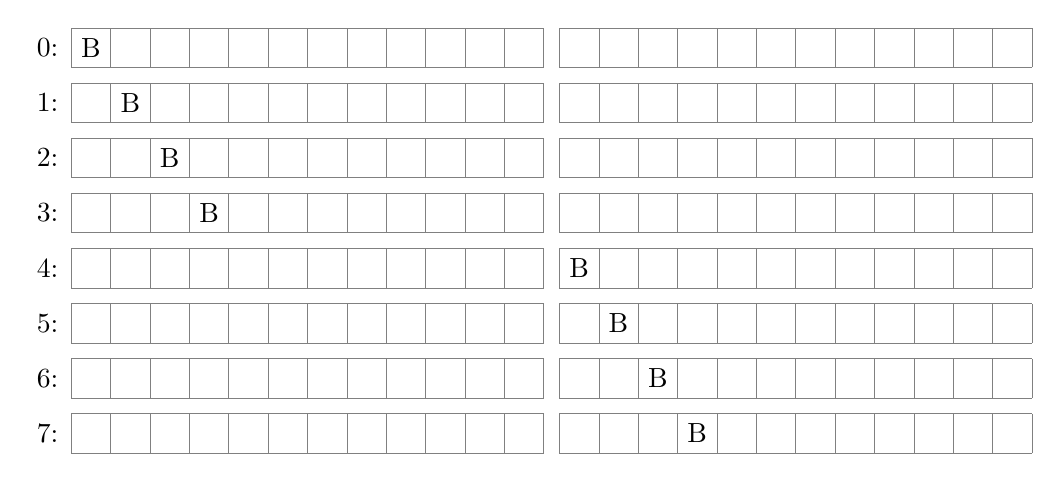
\begin{tikzpicture}
%   \foreach \i in {\xMin,...,\xMax} {
%       \draw [very thin,gray] (\i,\yMin) -- (\i,\yMax)  ;
%   }
%   \foreach \i in {\yMin,...,\yMax} {
%       \draw [very thin,gray] (\xMin,\i) -- (\xMax,\i) ;
%   }
    \foreach \j in {0,0.7,1.4,2.1,2.8,3.5,4.2,4.9} {
    \foreach \i in {0,0.5,1.0,1.5,2.0,2.5,3.0,3.5,4.0,4.5,5.0,5.5,6.0} {
        \draw [very thin,gray] (\i,\j) -- (\i,\j+0.5)  ;
        }

    \foreach \i in {\j,\j+0.5} {
        \draw [very thin,gray] (0,\i) -- (6.0,\i)  ;
        }


    \foreach \i in {0,0.5,1.0,1.5,2.0,2.5,3.0,3.5,4.0,4.5,5.0,5.5,6.0} {
        \draw [very thin,gray] (\i+6.2,\j) -- (\i+6.2,\j+0.5)  ;
        }

    \foreach \i in {\j,\j+0.5} {
        \draw [very thin,gray] (6.2,\i) -- (12.2,\i)  ;
        }
    }

    \node at (-0.3,0.25) {7: };
    \node at (-0.3,0.95) {6: };
    \node at (-0.3,1.65) {5: };
    \node at (-0.3,2.35) {4: };
    \node at (-0.3,3.05) {3: };
    \node at (-0.3,3.75) {2: };
    \node at (-0.3,4.45) {1: };
    \node at (-0.3,5.15) {0: };
    \node at (0.25,5.15) {B};
    \node at (0.75,4.45) {B};
    \node at (1.25,3.75) {B};
    \node at (1.75,3.05) {B};
    \node at (0.25+6.2,2.35) {B};
    \node at (0.75+6.2,1.65) {B};
    \node at (1.25+6.2,0.95) {B};
    \node at (1.75+6.2,0.25) {B};

  

\end{tikzpicture}

    \centering{}
  \caption{Process binding using openmpi and map-by ppr:8:node map-by ppr:4:socket on a node with two sockets and processors with each twelve cores}
\end{figure}


\begin{figure}[h]
  \centering
  \label{fig:binding3}
    \input{./img/map3.tikz.tex}
    \centering{}
  \caption{Process binding using openmpi and map-by ppr:8:node map-by ppr:4:socket:PE=3 on a node with two sockets and processors with each twelve cores}
\end{figure}

        Pinning of processes (picture), preliminary constraints by hardware and operating systems, identification of bottlenecks and explain possible workarounds, history and results of STREAM. Bandwidth as Bottleneck, how to calculate a Speedup estimate based on the measured bandwidth. PETSc Implementation of STREAM

\begin{figure} \centering
  \pgfplotsset{every axis/.append style={
      font=\large,
      line width=1pt,
  tick style={line width=0.8pt}}}
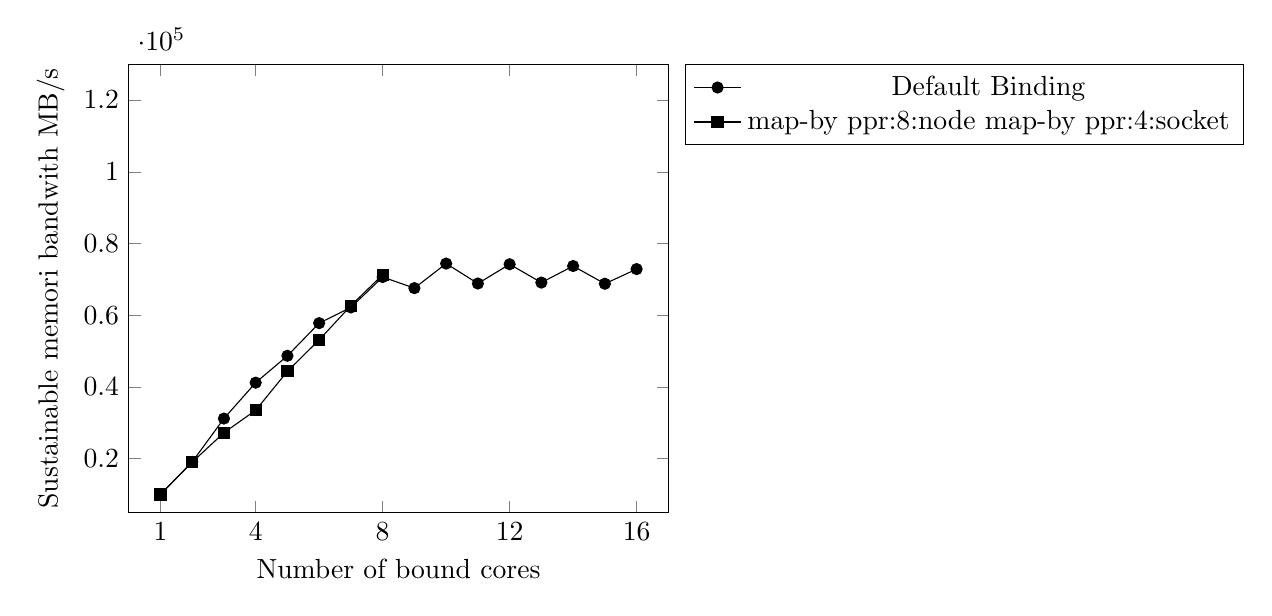
\begin{tikzpicture}
\begin{axis}[
    ylabel={Sustainable memori bandwith MB/s},
    xlabel={Number of bound cores},
    xtick={1,4,8,12,16},
    %ytick={1.7e-003,1.75e-3,1.8e-003,1.85e-3},
    %yticklabels={1.7E-3,1.75E-3,1.8E-3,1.85E-3},
    %ymin=1.65e-003,ymax=1.9e-003,
    xmin=0,xmax=17,
    ymin=0.5e4,ymax=1.3e5,
    legend pos=outer north east,
    %height=20cm,width=10cm
    ]
    \addplot[color=black,mark=*] coordinates {
        (1,10056.2733)
        (2,19114.3429)
        (3,31197.8399)
        (4,41210.0612)
        (5,48699.7232)
        (6,57803.5686)
        (7,62187.9785)
        (8,70658.3730)
        (9,67558.4259)
        (10,74413.8457)
        (11,68849.0631)
        (12,74223.3175)
        (13,69109.0762)
        (14,73729.0608)
        (15,68784.2613)
        (16,72872.4480) };
        \addlegendentry{Default Binding};
    \addplot[color=black,mark=square*] coordinates {
        (1 ,10044.2323)
        (2 ,19036.1755)
        (3 ,27258.6888)
        (4 ,33509.0570)
        (5 ,44386.9342)
        (6 ,53130.5978)
        (7 ,62695.4511)
        (8 ,71295.7113) };
        \addlegendentry{map-by ppr:8:node map-by ppr:4:socket}
\end{axis}
\end{tikzpicture}
\caption{Sustainable memory bandwidth for the STREAM benchmark (Triad) for different binding options on MPI1}
\end{figure}

\begin{figure} \centering
  \pgfplotsset{every axis/.append style={
      font=\large,
      line width=1pt,
  tick style={line width=0.8pt}}}
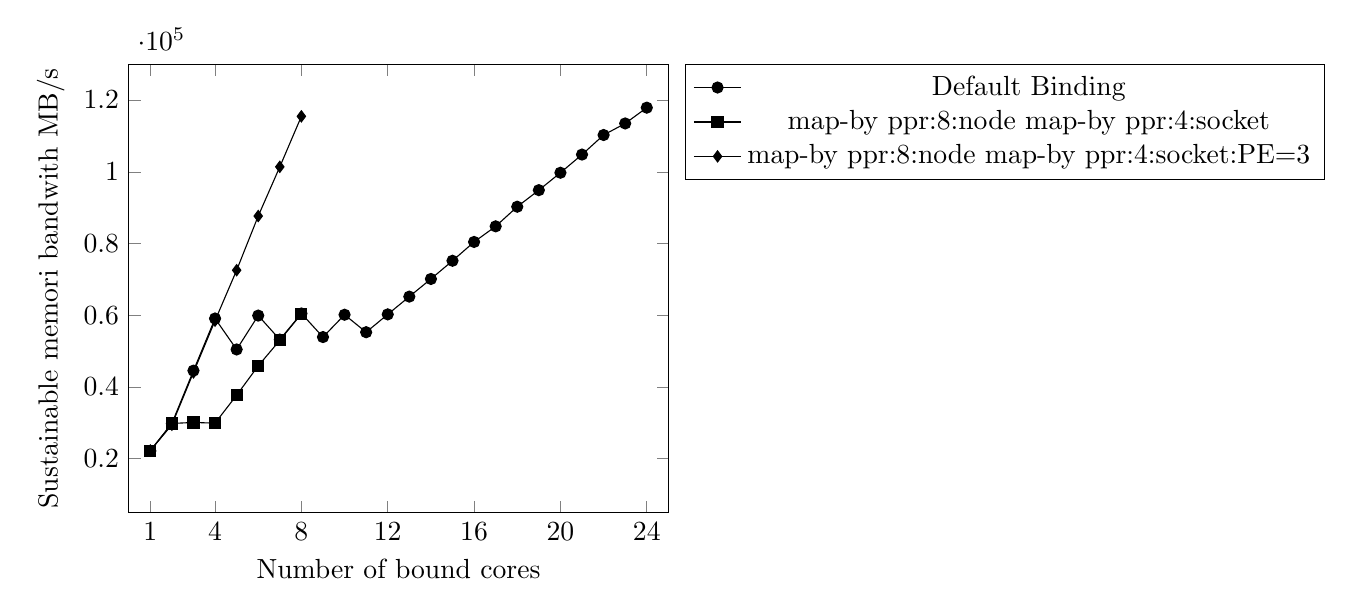
\begin{tikzpicture}
\begin{axis}[
    ylabel={Sustainable memori bandwith MB/s},
    xlabel={Number of bound cores},
    xtick={1,4,8,12,16,20,24},
    %ytick={1.7e-003,1.75e-3,1.8e-003,1.85e-3},
    %yticklabels={1.7E-3,1.75E-3,1.8E-3,1.85E-3},
    %ymin=1.65e-003,ymax=1.9e-003,
    legend pos=outer north east,
    xmin=0,xmax=25,
    ymin=0.5e4,ymax=1.3e5,
    %height=20cm,width=10cm
    ]
    \addplot[color=black,mark=*] coordinates {
           
      (1, 22201.8738 )
      (2,    29846.0651 )
      (3,    44558.8130 )
      (4,    59096.4718 )
      (5,    50460.8297 )
      (6,    59912.1938 )
      (7,    53222.7910 )
      (8,    60491.6764 )
      (9,    53922.4875 )
      (10,    60144.1732 )
      (11,    55273.7403 )
      (12,    60248.1185 )
      (13,    65200.5600 )
      (14,    70118.7250 )
      (15,    75192.3175 )
      (16,    80439.8917 )
      (17,    84793.6761 )
      (18,    90263.9931 )
      (19,    94881.4421 )
      (20,    99735.0136 )
      (21,   104804.3772 )
      (22,   110256.7754 )
      (23,   113478.3185 )
    (24,   117880.3816 ) };
     \addlegendentry{Default Binding};
     \addplot[color=black,mark=square*] coordinates{
       (1, 22211.6717)
       (2, 29836.1141)
       (3, 30113.6704)
       (4, 29919.5219)
       (5, 37713.7578)
       (6, 45888.1496)
       (7, 53019.1276)
     (8, 60375.4338) };
     \addlegendentry{map-by ppr:8:node map-by ppr:4:socket};
     \addplot[color=black,mark=diamond*] coordinates{
       (1, 22265.7147)
       (2, 29467.1111)
       (3, 44064.6918)
       (4, 58503.9143)
       (5, 72560.6185)
       (6, 87667.8368)
       (7,101388.5503)
     (8,115464.4300) };
     \addlegendentry{map-by ppr:8:node map-by ppr:4:socket:PE=3};
\end{axis}
\end{tikzpicture}
\caption{Sustainable memory bandwidth for the STREAM benchmark (Triad) for different binding options on MPI1}
\end{figure}

      \subsubsection{Discussion of Results for Parallel Efficiency}
      \subsubsection{Speedup Measurement for Analytic Test Cases}

    \subsection{Test Cases with Varying Degree of Non-Linearity}
      
      As Peric says I want to prove that the higher the non-linearity of NS, the better relative convergence rates can be achieved with a coupled solver. Fi

      \subsubsection{Transport of a Passive Scalar -- Forced Convection}
      \subsubsection{Buoyancy Driven Flow -- Natural Convection}
      \subsubsection{Flow with Temperature Dependent Density -- A Highly Non-Linear Test Case}
        Maybe I could consider two test cases, one with oscillating density and one with a quadratic polynomial. Interesting would be also to consider the dependence of convergence on another scalar transport equation

    \subsection{Realistic Testing Scenarios -- Benchmarking}
        Also consider simple load balancing by distributing matrix rows equally
      
      \subsubsection{Flow Around a Cylinder 3D -- Stationary}
        Describe Testing Setup (Boundary conditions and grid). Present results and compare them with literature.
      \subsubsection{Flow Around a Cylinder 3D -- Instationary}
        \begin{itemize}
          \item\url{http://www.featflow.de/en/benchmarks/cfdbenchmarking/flow/dfg_flow3d/dfg_flow3d_configuration.html}
        \end{itemize}
        Describe Testing Setup (Boundary conditions and grid). Present results and compare them with literature.

      \subsubsection{Heat-Driven Cavity Flow}
        \begin{itemize}
          \item \url{http://www.featflow.de/en/benchmarks/cfdbenchmarking/mit_benchmark.html}
        \end{itemize}
        Describe Testing Setup (Boundary conditions and grid). Present results and compare them with literature.
    \subsection{Realistic Testing Scenario -- Complex Geometry}

  \section{Conclusion and Outlook}
\label{sec:conclusion}

In the present thesis a fully coupled solution algorithm for the Navier-Stokes equations with a finite-volume method on co-located, locally refined block-structured grids was implemented. The main difference of this algorithm compared to the commonly used segregated solution algorithms was the implicit pressure-velocity coupling. The pressure-velocity coupling is a characterizing aspect of solution algorithms for Navier-Stokes equations with the potential to significantly reduce the time for computation. Furthermore the solution algorithm was extended to solve for buoyancy driven flows, by using an implicit Boussinesq approximation in the momentum balances to achieve velocity-to-temperature coupling and a semi-implicit Newton-Raphson linearization to realize implicit temperature-to-velocity/pressure coupling.

The CAFFA solver framework, that was extended during this thesis was verified using a grid convergence study and a three-dimensional manufactured solution for the velocities, the pressure and the temperature. Further studies on the segregated solution algorithm showed, that a special modification of the widely used Rhie-Chow momentum interpolation scheme is necessary to calculate results that are independent of the under-relaxation factor and thus comparable with the results obtained with a fully coupled solution algorithm. In the implementation of the algorithm the further use on high performance computers was considered, using the PETSc library for parallelisation of the involved data structures and solving the resulting linear systems with solvers and preconditioners provided from the same toolkit.

A comparison study was performed dealing with the effect of implicit pressure-velocity coupling in the solution of the Navier-Stokes equations. Parallel performance measurements showed that for the implementation of the segregated and the coupled solution algorithm scalable program behaviour is possible for high numbers of involved unknowns. Performance studies on flows through complex geometries showed that the fully couple solution algorithm outperforms the segregated solution algorithm. 

The analyses regarding the different degrees of velocity-to-temperature and temperature-to-velocity/pressure coupling showed that the implicit temperature-to-velocity/pressure coupling is the key aspect of maintaining high efficiency regarding the computation time for flow problems involving temperature transport and strong coupling between the velocities, the pressure and the temperature.

The present thesis revealed different starting points to further examine the effects of coupled solution algorithms in the context of finite-volume flow solvers. In the present thesis only stationary problems were solved. Due to the moderate Rayleigh number for the heated cavity test case a stationary solution existed. By increasing the Rayleigh number the coupling between the velocities, the pressure and the temperature would get stronger, however the flow will get instationary. A further investigation could examine if coupled solution methods maintain the higher efficiency compared to segregated solution algorithms when applied to instationary flows.

In this thesis a temperature equation was successfully coupled to the modeling equations of a fluid. One straightforward application of the solver would deal with conjugate heat transfer problems. On the other side in practice there exist other similar transport equations that exhibit strong coupling to the velocities. Examples are the scalar transport of volume fractions, when multiphase flows are solved with Volume-of-Fluid methods or turbulent flows, which depending on the turbulence model involve further scalar quantities that are strongly coupled to the velocities. Subsequent studies could examine if for the corresponding transport equations a implict coupling method could be efficiently implemented.

All linear systems surging from the discretization process of the coupled system of partial differential equations were solved using black-box implementations of the available solvers in the PETSc library. As studies on finite-volume \cite{klaij13,darwish09,mangani14} and finite-element \cite{brown12,elman03,elman08,silvester01,turek02,mcinnes14} discretizations show, a lot of information has not been used in the solution process of the linear system yet, which imposes a barrier on performance. In order to exploit the coupling and the structure of the linear systems two different approaches can be considered. On approach features so called \emph{physics-based} preconditioners as the SIMPLE preconditioner or other Schur-type preconditioners introduced in \cite{klaij13,elman08}. These kind of preconditioners accelerate the solution of the linear systems by taking into account the matrix structure as it is presented in figure \ref{fig:nointerlacemat}. At the moment further active research is needed to develop preconditioners for fully coupled systems surging from finite-volume discretizations. Another approach that additionally maintains high scalability of the solution algorithm of the resulting linear systems have been presented in \cite{darwish09,mangani14}. In these approaches algebraic multigrid methods are constructed, that, different to the GAMG preconditioner in PETSc, take into account the matrix structure.

As the studies in the present thesis showed, segregated solution algorithms can perform well compared to fully coupled solution algorithms for smaller numbers of unknowns. Furthermore due to the lower requirements on system memory, the problems that can be solved with segregated solution algorithms may for high numbers of unknowns not be computable with fully coupled solution algorithms. Especially for flows involving temperature transport many other implementations of segregated solution algorithms exist, whose performance has not been compared with a coupled solution method. Examples can be found in \cite{liu84,oliveira01}.



%testing purposes
    \nocite{*}

\clearpage
\addcontentsline{toc}{section}{References}
\bibliography{bib/masterthesis.articles,bib/masterthesis.books}
%if using biblatex
%\printbibliography[title={Book references},type=book]
%\printbibliography[title={Article references},type=article]
%\printbibliography[title={Other references}, nottype=article, nottype=book]
\end{document}
